\chapter{Programmieren des TransistorTesters}

\section{Konfigurieren des TransistorTesters}
\label{sec:config}
Die ganze Software des TransistorTesters ist im Quellcode verfügbar.
Die Übersetzung der Module wird mit einer \lname{Makefile} gesteuert. Die Entwicklung wurde
auf einem Ubuntu Linux mit den GNU-Werkzeugen (GNU toolchain, gcc version 4.5.3) durchgeführt.
Es sollte möglich sein, ohne Schwierigkeiten andere Linux-Betriebssysteme zu benutzen.
Um die übersetzen Daten in den Flash-Speicher oder den EEPROM-Speicher zu laden, wird das
Programm \lcmd{avrdude} \cite{avrdude} (Version 6.3) von der \lname{Makefile} benutzt, wenn man \lcmd{make upload} aufruft.
Das Programm \lcmd{avrdude} ist für Linux und Windows verfügbar.
Der GNU C-Kompiler wird auch von der AVR-studio-Software unter Windows oder von
der WinAVR \cite{winavr1},\cite{winavr2} Software benutzt.
Sie können die Programmdaten (.hex und .eep) auch mit anderen Programmen in den ATmega laden,
aber nur meine \lname{Makefile}-Version stellt sicher, dass die richtigen Daten in den gewählten Prozessor gelangen.
Avrdude lädt Daten nur in den ATmega, wenn die Signaturbytes des angeschlossenen ATmega gleich mit dem ausgewählten sind.
Wenn Sie die \lname{Makefile} ändern, wird die Software komplett neu übersetzt, wenn man \lcmd{make} oder
\lcmd{make upload} aufruft.
Die Software, die für einen ATmega8 übersetzt wurde, läuft nicht auf einem ATmega168.
Die Software, die für einen ATmega328 übersetzt wurde, läuft nicht auf einem ATmega168.
Eine Ausnahme bildet Software, die für einen ATmega168 übersetzt wurde. Diese Programmdateien
sind auch für einen ATmega328 brauchbar.
Seien Sie vorsichtig, wenn Sie nicht das mitgelieferte \lname{Makefile} benutzen.

Mit den entsprechenden Optionen ist die Software auch auf dem unveränderten Hardware-Entwurf von
Markus F. lauffähig (PARTNO=m8 , \textbf{keine} NO\_AREF\_CAP und \textbf{keine} PULLUP\_DISABLE Option).
Die Taktrate kann mit den fuses auch auf \(8MHz\) gestellt werden, dazu ist kein Quarz erforderlich!


Die folgenden Optionen der \lname{Makefile} sind verfügbar, um die Software für den Tester zu konfigurieren:

\begin{description} \setlength{\itemsep}{0em}
  \item[PARTNO] beschreibt den Ziel-Prozessor:\\
         m8 = ATmega8\\
         m168 or m168p = ATmega168\\
         m328 or m328p = ATmega328\\
         m644 or m644p = ATmega644\\
         m1284p        = ATmega1284\\
         m1280         = ATmega1280\\
         m2560         = ATmega2560\\
    Beispiel: PARTNO = m168

  \item[UI\_LANGUAGE] gibt die Sprache für den Tester an:\\
    LANG\_BRASIL, LANG\_CZECH, LANG\_DANISH, LANG\_DUTCH, LANG\_ENGLISH, \\
    LANG\_GERMAN, LANG\_HUNGARIAN, LANG\_ITALIAN, LANG\_LITHUANIAN, \\
    LANG\_POLISH, LANG\_RUSSIAN, LANG\_SLOVAK, LANG\_SLOVENE, \\
    LANG\_SPANISH, und LANG\_UKRAINIAN sind derzeit verfügbar.
 Für die russische und ukrainische Sprache ist ein LCD mit kyrillischem Zeichensatz erforderlich.\\
    Beispiel: UI\_LANGUAGE = LANG\_ENGLISH

  \item[LCD\_CYRILLIC] wird nur gebraucht, wenn man ein LC-Display mit kyrillischem Zeichensatz benutzt.
Die Zeichen \(\mu\) und \(\Omega\) sind im kyrillischen Zeichensatz nicht enthalten.
Wenn Sie diese Option angeben, werden beide Zeichen von der Software in das LCD geladen.
Setzen sie diese Option, wenn bei der Ausgabe falsche Zeichen anstelle von \(\mu\) oder \(\Omega\) erscheinen.\\
Beispiel: CFLAGS += -DLCD\_CYRILLIC

  \item[LCD\_DOGM] muss angegeben werden, wenn ein LCD mit ST7036-Controller (Typ DOG-M) zur Anzeige verwendet wird.
Der LCD-Kontrast wird dann mit Software-Befehlen eingestellt.
Falls sie den Kontrast zu weit verstellt haben, daß auf dem Display nichts mehr zu erkennen ist,
können sie zunächst versuchen, ob nicht bei seitlicher Sicht auf das Display doch noch etwas zu erkennen ist.
sonst muß das EEprom neu beschrieben werden, um den Kontrastwert zurückzusetzen.\\
Beispiel: CFLAGS += -DLCD\_DOGM

  \item[FOUR\_LINE\_LCD] kann bei einem 4x20-Zeichen-Display verwendet werden, um den Platz auf dem Display
besser auszunutzen. Zusätzliche Parameter, welche sonst nur kurz in Zeile 2 angezeigt werden, werden dann in
den Zeilen 3 und 4 angezeigt.\\
Beispiel: CFLAGS += -DFOUR\_LINE\_LCD

  \item[DD\_RAM\_OFFSET] Bei einigen Text-Displays werden andere DD-RAM Startadressen für den Zeilenanfang
benutzt. Normalerweise beginnt die erste Zeile bei der DD-RAM Adresse 0. Bei einigen Displays wie TC1604
oder TC1602 beginnt die Zeile 1 aber bei der Adresse 128 (0x80).
Das kann mit dieser Option berücksichtigt werden.\\
Beispiel: CFLAGS += -DDD\_RAM\_OFFSET = 128

  \item[WITH\_LCD\_ST7565] Diese Option muss verwendet werden, wenn ein 128x64 Pixel LCD mit serieller
Schnittstelle angeschlossen ist.
Für diesen Displaytyp müssen weitere Optionen gesetzt werden, die in Tabelle~\ref{tab:cod-display} 
beschrieben werden.
Anstelle des ST7565-Controllers kann auch zum Beispiel der ähnliche SSD1306-Controller konfiguriert werden.
Dafür muss diese Option auf 1306 gesetzt werden.
Ein PCF8812 oder PCF8814 Controller wird ebenfalls unterstützt, wenn diese Option richtig gesetzt wird.
Auch ein Display mit ST7920 oder NT7108 Controller kann angeschlossen werden.
Für den NT7108 Controller muß ein
zusätzlicher Seriell-Parallel Wandler 74HC(T)164 oder 74HC(T)595 verwendet werden.\\
Beispiel: WITH\_LCD\_ST7565 = 1 

 \item[LCD\_INTERFACE\_MODE] Beim SSD1306-Controller kann anstelle des Standard-SPI (4-Wire) Interface auch das
I\textsuperscript{2}C-Interface benutzt werden. Dafür muss diese Option auf 2 gesetzt werden.
Für den ST7920 Controller kann ein spezieller serieller Anschluß mit dem Setzen dieser Option auf 5
unterstützt werden.
Wenn nur eine Anschlußmöglichkeit vorgesehen ist, braucht die Konstante LCD\_INTERFACE\_MODE nicht gesetzt werden.
Alle bisher möglichen Werte für LCD\_INTERFACE\_MODE und WITH\_LCD\_ST7565 sind in Tabelle~\ref{tab:cod-display} aufgeführt.\\

\begin{table}[H]
  \begin{center}
    \begin{tabular}{| c | c | c | c|}
    \hline
 Display-Typ        &  Interface     & WITH\_LCD\_ST7565 &  LCD\_INTERFACE\_MODE \\
    \hline
    \hline
  Character 16x2,   & 4-Bit parallel &  disabled (0)      & disabled (1) \\
  Character 20x4    & 4-Wire SPI     &                    &    4   \\
                  & I\textsuperscript{2}C &               &    2   \\
    \hline
  Graphic ST7565    & 4-Wire SPI      & 1 or 7565          & disabled (4) \\
    \hline
  Graphic ST7565  & I\textsuperscript{2}C & 1 or 7565     &   2 \\
    \hline
  Graphic SSD1306   & 4-Wire SPI      & 1306               & disabled (4) \\
    \hline
  Graphic SSD1306 & I\textsuperscript{2}C & 1306          &   2 \\
    \hline
  Graphic ST7920    & 4-Bit parallel  & 7920              & disabled (1) \\
    \hline
  Graphic ST7920    & 2-Bit serial    & 7920               &  5 \\
    \hline
  Graphic NT7108    & 8-Bit parallel  & 7108              & disabled (6) \\
  oder KS0108       &    + 74HCT164   &                   &      \\
    \hline
  Graphic PCF8812   & 4-Wire SPI      & 8812              & disabled (4) \\
    \hline
  Graphic PCF8814   & 4-Wire SPI      & 8814              & disabled (4) \\
                  & I\textsuperscript{2}C & 8814          &   2 \\
                    & 3-line          & 8814              &   3 \\
    \hline
  Graphic ILI9163   & 4-Wire SPI      & 9163              & disabled (4) \\
  128x128 Color     &                 &                   &              \\
    \hline
  Graphic ST7735    & 4-Wire SPI      & 7735              & disabled (4) \\
  128x160 Color     &                 &                   &              \\
    \hline
    \end{tabular}
  \end{center}
  \caption{Kennzahlen für Controller und  Art der Schnittstelle}
  \label{tab:cod-display}
\end{table}

Die Werte in Klammern werden nur Software intern benutzt und sind hier nur zur Information genannt.
Man sollte die Werte in den Klammern nicht hier in der \lname{Makefile} setzen.\\
Beispiel: CFLAGS += -DLCD\_INTERFACE\_MODE=2

  \item[LCD\_SPI\_OPEN\_COL] Mit der Option LCD\_SPI\_OPEN\_COL werden die Datensignale der SPI-Schnittstelle
nicht nach VCC direkt geschaltet.
Die Signale werden nur nach GND geschaltet, für die \inquotes{high} Signale werden die \inquotes{Pull-Up} Widerstände
des ATmega benutzt.
Für das Signal \inquotes{Reset} wird aber ein externer Pull-Up Widerstand benötigt, wenn die Option PULLUP\_DISABLE
gesetzt ist. Für die anderen SPI Signale werden die internen Pull-Up Widerstände vorübergehend benutzt,
wenn die Option PULLUP\_DISABLE gesetzt ist.
Beispiel: CFLAG += -DLCD\_SPI\_OPEN\_COL

 \item[LCD\_I2C\_ADDR] Die I\textsuperscript{2}C-Adresse des SSD1306-Controllers kann durch Vorbesetzen der Adresse LCD\_I2C\_ADDR
auf 0x3D geändert werden.\\
Beispiel: CFLAGS += -DLCD\_I2C\_ADDR=0x3d

  \item[LCD\_ST7565\_RESISTOR\_RATIO] Mit dieser Option wird das Widerstands-Teilerverhältnis für den
Spannungsregler des ST7565-Controllers eingestellt. Brauchbare Werte liegen im Allgemeinen zwischen 4 und 7.
Einstellbar sind Werte zwischen 0 und 7.\\
Beispiel: LCD\_ST7564\_RESISTOR\_RATIO = 4

  \item[LCD\_ST7565\_H\_FLIP] Mit dieser Option kann die Anzeige horizontal umgedreht werden.\\
Beispiel: CFLAGS += LCD\_ST7565\_H\_FLIP = 1

  \item[LCD\_ST7565\_H\_OFFSET] Diese Option kann den für die Ausgabe benutzten Speicher an das Anzeigefenster des
 Displays anpassen. Der Controller benutzt mehr horizontale Pixel (132) als angezeigt (128) werden.
 Ein Wert von 0, 2 oder 4 kann je nach verwendetem Display-Modul für eine korrekte Darstellung notwendig sein.\\
Beispiel: CFLAGS += LCD\_ST7565\_H\_OFFSET = 4

  \item[LCD\_ST7565\_V\_FLIP] Mit dieser Option kann die Anzeige vertikal umgedreht werden.\\
Beispiel: CFLAGS += LCD\_ST7565\_V\_FLIP = 1

  \item[VOLUME\_VALUE] Hier kann man den Kontrastwert für ST7565 oder SSD1306 Controller voreinstellen.
Der Wert kann für den ST7565 Controller zwischen 0 und 63 liegen.
Für den SSD1306 Controller sind Werte zwischen 0 und 255 erlaubt.\\
Beispiel: CFLAGS += -DVOLUME\_VALUE = 25

  \item[LCD\_ST7565\_Y\_START] Mit dieser Option kann die erste Zeile vertikal richtig gesetzt werden.
Bei einigen Display-Varianten ist die erste Zeile in die Bildmitte verschoben.
Bei diesen Displays wird die erste Zeile wieder an den oberen Rand verschoben, 
wenn diese Option auf 32 (halbe Bilschirmhöhe) gesetzt wird.\\
Beispiel: CFLAGS += -DLCD\_ST7565\_Y\_START = 32

  \item[LCD\_CHANGE\_COLOR] Diese Option erweitert die Menüfunktionen um die Möglichkeit,
die Hindergrundfarbe und die Vordergrundfarbe wählen zu können. Wenn die Option auf
den Wert 2 gesetzt wird, werden die Farben blau und rot vertauscht.
Diese Option kann nur für Farbdisplays (Controller ST7735 oder ILI9193) gewählt werden.\\
Beispiel: CFLAGS += -DLCD\_CHANGE\_COLOR=1

 \item[LCD\_BG\_COLOR] Mit dieser 16-Bit Zahl kann eine Farbe für den Hintergrund gewählt werden.
Normalerweise sind die oberen 5 Bit für die Farbe rot, die mittleren 6 Bit für die Farbe grün
und die unteren 5 Bit für die Farbe blau vorgesehen. Manchmal sind aber die Bits für die Farben 
rot und blau vertauscht.
Diese Option kann nur für Farbdisplays (Controller ST7735 oder ILI9193) gewählt werden.\\
Beispiel: CFLAGS += -DLCD\_BG\_COLOR=0x000f

 \item[LCD\_FG\_COLOR] Mit dieser 16-Bit Zahl kann eine Farbe für den Vordergrund gewählt werden.
Das Beispiel wählt weiss als Farbe für Text und Symbole aus.
Diese Option kann nur für Farbdisplays (Controller ST7735 oder ILI9193) gewählt werden.\\
Beispiel: CFLAGS += -DLCD\_FG\_COLOR=0xffff

  \item[FONT\_8X16] Für den ST7565 controller sollte ein Font ausgewählt werden.
Auswählbar sind die Fonts mit der Variablen FONT\_ mit angehängter Größe (Breite x Höhe).
iDerzeit sind 6X8, 8X8, 7X12, 8X12, 8X12thin, 8X14 8X15, 8X16 und 8X16thin.
Die Fontgröße 8x16 oder 8X16thin ist die effizienteste Wahl für das graphische 128x64-LCD.\\
Beispiel: CFLAGS += FONT\_8X16

 \item[BIG\_TP] Die Pinnummern bei der graphischen Darstellung können mit dieser Option größer dargestellt werden.\\
Beispiel: CFLAGS += BIG\_TP

 \item[INVERSE\_TP] Mit dieser Option werden die Pinnummern in der graphischen Darstellung invers (schwarz auf weiß) dargestellt.
Weil für die Darstellung ein Rand benötigt wird, kann diese Option nicht mit der Option BIG\_TP kombiniert werden.\\
Beispiel: CFLAGS += INVERSE\_TP

  \item[STRIP\_GRID\_BOARD] Diese Option passt die Software an eine andere Pinbelegung von Port~D für Streifenleiterplatinen an.
Die Einzelheiten findet man im Hardwarekapitel \ref{sec:hardware} auf Seite~\pageref{sec:hardware}.
Mit dieser Option werden auch alternative Belegungen der ATmega Pins für graphische Displays gewählt.
Für die chinesische \inquotes{T5} Platine muß die Option STRIP\_GRID\_BOARD auf 5 gesetzt werden.
Bei den Alternativen für die graphischen Displays bleibt die Belegung  des Tastensignals unverändert.\\
Beispiel: CFLAGS += -DSTRIP\_GRID\_BOARD

  \item[WITH\_MENU] aktiviert eine Menüfunktion für einen ATmega328. Man kann einige Zusatzfunktionen über ein
Auswahlmenü benutzen, welches man über einen langen Tastendruck (\textgreater~0,5s) erreichen kann.
Wenn die Menüfunktion eingeschaltet ist, wird beim automatischen Selbsttest-Start mit kurzgeschlossenen Testpins
 nur der Kalibrationsteil des Selbsttests ausgeführt.
Die Tests T1-T7 werden nur beim Selbsttest ausgeführt, der als Menüfunktion ausgewählt werden kann.\\
Beispiel: CFLAGS += -DWITH\_MENU

 \item[MAX\_MENU\_LINES]
Diese Option gibt eine maximale Zeilenzahl für die gezeigte Auswahl der Menüfunktionen an.
Normalerweise ergibt sich die Zahl der Zeilen über die vorhandene Zeilenzahl des Displays.
Da normalerweise mehr Funktionen ausgewählt werden können als auf dem Display Zeilen zur Verfügung stehen,
wird die Auswahl zyklisch ausgetauscht.
Die Aufbereitung des Displayinhalts bei dem zyklischen Austausch braucht speziell bei großen Farbdisplays
mit vielen Zeilen erhebliche Zeit.
Durch die Begrenzung der Zeilenzahl mit dieser Option kann die Ausgabezeit bei der Menüauswahl deutlich reduziert werden
und so die Bedienung beschleunigt werden.
Der Wert für diese Option ist mit 5 vorbesetzt.\\
Beispiel: CFLAGS += -DMAX\_MENU\_LINES=3

  \item[WITH\_ROTARY\_SWITCH] Die Menüfunktion kann leicher bedient werden, wenn ein Impulsdrehgeber als Erweiterung
benutzt wird.
Für die Details der notwendigen Erweiterung sehen Sie bitte die Beschreibung~\ref{fig:RotExt} im Hardwarekapitel.
Wenn der Impulsdrehgeber die gleiche Anzahl von Raststellungen wie Impulse für jede Umdrehung hat,
muss die Option WITH\_ROTARY\_SWITCH auf 2 gesetzt werden.
Wenn der Impulsdrehgeber doppelt so viele Raststellungen hat, muss die Option WITH\_ROTARY\_SWITCH auf 1 gesetzt werden.
Das Setzen der Option WITH\_ROTARY\_SWITCH auf 5 wählt die höchste Auflösung für den Impulsdrehgeber.
Jeder Zyklus der beiden Schalter-Zustände wird als 4 gezählt. Normalerweise ist diese Einstellung nur für
Impulsdrehgeber ohne Raststellung sinnvoll.
Ein Setzen der Option WITH\_ROTARY\_SWITCH auf 4 ist notwendig für die korrekte Behandlung von zwei separaten
Rauf (Up) und Runter (Down) Tastern, die anstelle der beiden Schalter eines Impulsdrehgebers eingebaut sind.
Verwenden Sie nicht die Einstellung 4 mit normalen Impulsdrehgebern!\\
Beispiel: CFLAGS += -DWITH\_ROTARY\_SWITCH=1

  \item[CHANGE\_ROTARY\_DIRECTION] Man kann die erkannte Drehrichtung des Impulsdrehgebers durch Vertauschen
der beiden Schalter-Signale oder durch Setzen dieser Option ändern.
Beispiel: CFLAGS += -DCHANGE\_ROTARY\_DIRECTION

 \item[WITH\_SELFTEST] Wenn Sie diese Option angeben, baut die Software eine Selbsttest-Funktion ein, die gestartet wird
wenn Sie alle drei Prüfspitzen verbinden und eine Messung starten.\\
Beispiel: CFLAGS += -DWITH\_SELFTEST

  \item[NO\_COMMON\_COLLECTOR\_HFE] verhindert die hFE-Messung von Transistoren in der Kollektorschaltung.
So können Sie Speicher sparen, um die erweiterten Selbsttest-Routinen T1 bis T7 für den ATmega168-Prozessor zu ermöglichen.
Standardmäßig sind beide Schaltungen für die hFE-Messung eingeschaltet,
aber dann ist kein Platz im Programmspeicher des ATmega168 für die erweiterten Selbsttests.\\
Beispiel: CFLAGS += -DNO\_COMMON\_COLLECTOR\_HFE

  \item[NO\_COMMON\_EMITTER\_HFE] schaltet die hFE-Messung von Transistoren in Emitterschaltung ab.
So können Sie Speicher sparen, um die erweiterten Selbsttest-Routinen T1 bis T7 für den ATmega168-Prozessor zu ermöglichen.
Standardmäßig sind beide Schaltungen für die hFE-Messung eingeschaltet,
aber dann ist kein Platz im Programmspeicher des ATmega168 für die erweiterten Selbsttests.\\
Beispiel: CFLAGS += -DNO\_COMMON\_EMITTER\_HFE

  \item[NO\_TEST\_T1\_T7] Diese Option verhindert die Ausführung der Selbsttest Teile T1 bis T7.
Diese Tests sind nützlich um Fehler in der Schaltung wie falsche Messwiderstände oder Isolationsprobleme zu finden.
Wenn Ihre Schaltung fehlerfrei ist, können Sie die Selbsttest-Teile T1 bis T7 durch das Setzen dieser Option weglassen, um eine
schnellere Kalibration zu erreichen.
Bei eingeschalteter Menüfunktion werden die Selbsttest-Teile T1 bis T7 nur bei Aufruf der Menüfunktion \inquotes{Selbsttest} ausgeführt.
Der ATmega168-Prozessor benutzt die Selbsttest Teile T1 bis T7 nicht, wenn beide Messmethoden für die hFE-Bestimmung benutzt werden.\\
Beispiel: CFLAGS += -DNO\_TEST\_T1\_T7

  \item[AUTO\_CAL] Der Nullabgleich für die Kondensatormessung wird beim
Selbsttest zusätzlich ins EEPROM geschrieben und ist damit für die weiteren Messungen abgeglichen.
Wenn nach dem Nullabgleich der Kondensatormessung ein Kondensator mit einer Kapazität zwischen \(100nF\) und \(20\mu F\) an Pin~1 und Pin~3 
angeschlossen wird, wird auch der Offset des analogen Komparators und die Skalierung für die AUTOSCALE\_ADC
Umschaltung auf die interne Spannungsreferenz ermittelt und ins EEPROM geschrieben.
Die Port-Ausgangswiderstände werden zu Beginn jeder Messung neu bestimmt. \\
Beispiel: CFLAGS += -DAUTO\_CAL

  \item[SHORT\_UNCAL\_MSG] Bei Prozessoren mit mindestens 32K Flash  wird nach einem Bauteiletest ein Hinweis auf einen unkalibrierten Zustand
des Testers gegeben. Normalerweise folgt dann eine kurze Anleitung, wie die Kalibration durchzuführen ist.
Diese Anleitung wird nicht ausgegeben, wenn die Option SHORT\_UNCAL\_MSG gesetzt wird.
Dann bleibt es bei einem einzeiligen Hinweis auf den unkalibrierten Zustand. 
Dies spart einerseits etwas Platz in Flash-Speicher und andererseits Ausgabezeit für Benutzer,
die ohnehin wissen, wie kalibriert wird.\\
Beispiel: CFLAGS += -DSHORT\_UNCAL\_MSG

 \item[NO\_ICONS\_DEMO]
Diese Option schaltet die zusätzliche Demonstration der Symbole und die Ausgabe des Zeichensatzes bei der Menüfunktion
\inquotes{Zeige Daten} ab.
Dies spart Platz im Flash-Speicher und auch Ausgabezeit für den Nutzer.\\
Beispiel: CFLAGS += -DNO\_ICONS\_DEMO

 \item[WITH\_ROTARY\_CHECK]
Diese Option schaltet die zusätzliche Menüfunktion für den Test eines Impulsdrehgebers frei.
Dieser Test testet einen Impulsdrehgeber, der an TP1,TP2 und TP3 angeschlossen wird.
Bitte beachten Sie, daß nicht der eingebaute Impulsdrehgeber des Testers getestet wird!
Aber ein solcher Impulsdrehgeber kann mit der Option WITH\_ROTARY\_SWITCH auch zur Bedienung des Testers eingesetzt werden.\\
Beispiel: CFLAGS += -DWITH\_ROTARY\_CHECK

 \item[NO\_FREQ\_COUNTER]
Mit dieser Option wird die Frequenzzähler Funktion des Testers abgewählt.
Dies ist besonders dann sinnvoll, wenn der benutzte Pin PD4 (ATmega328) nicht zusammen mit
dem Anschluß des Displays benutzt werden kann.
Der entsprechende Eintrag in der Liste der Menüfunktionen erscheint dann nicht mehr und es
wird auch Flash-Speicherplatz gespart.\\
Beispiel: CFLAGS += -DNO\_FREQ\_COUNTER

 \item[WITH\_FREQUENCY\_DIVIDER]
Mit dieser Option wird das Menü um einen einstellbaren Vorteiler für den Frequenzzähler erweitert.
Das Teilerverhältnis kann auf 1:1, 1:2, 1:4, 1:8, 1:16, 1:32, 1:64 und 1:128 eingestellt werden.
Diese Option ist nur sinnvoll, wenn an den Frequenzeingang ein externer Vorteiler angeschlossen wird.
Die bei der Messung angezeigten Frequenzen und Perioden berücksichtigen das eingestellte Teilerverhältnis.\\
Beispiel: CFLAGS += -DWITH\_FREQUENCY\_DIVIDER

 \item[NO\_FREQUENCY\_SWITCH]
Mit dieser Option wird die Umschaltung des Frequenzeingangs der ATmega644/ATmega1284 Schaltung nicht unterstützt.
Die LF- und HF-Quarz Messung wird mit dieser Option nicht unterstützt.\\
Beispiel: CFLAGS += -DNO\_FREQUENCY\_SWITCH=1

\item[PWM\_SERVO] 
wählt eine spezielle PWM Erzeugung zum Testen von Modellbau Servos anstelle der allgemeinen PWM Erzeugung.\\
Beispiel: CFLAGS += -DPWM\_SERVO=1

  \item[WITH\_SamplingADC] Mit dieser Funktion wird in bestimmten Fällen die Sampling-Methode für den ADC angewendet.
Durch Verschieben der Abtastzeit des ADC kann für wiederholbare Signale die Signalform mit einem Zeitabstand
von einem Prozessortakt oder auch 4 oder 16 Prozessortakte abgetastet werden. Dadurch kann die Ladefunktion von
Kondensatoren unter \(100pF\) so vermessen werden, daß sich eine Auflösung von \(0.01pF\) bei \(16MHz\) Prozessortakt ergibt.
Mit den gleichen Methode kann die Schwingfrequenz bei kleinen Spulen unter \(2mH\) mit einem parallelgeschalteten
Kondensator gemessen werden. Wenn die Kapazität des Parallel-Kondensators bekannt ist, kann die Induktivität aus
der Schwingfrequenz mit hoher Auflösung bestimmt werden. Als Nebenprodukt kann auch die Güte der Spule aus dem
Schwingverhalten geschätzt werden. Freigeschaltet werden diese Funktionen mit der Option WITH\_SamplingADC.
Bei der Kalibration werden dann sowohl zusätzlich die Nullkapazitäten mit der Samplingmethode zusätzlich bestimmt,
als auch die Kapazität eines Parallel-Kondensators vermessen für die spätere Bildung eines Schwingkreises mit einer unbekannten Spule.\\
Beispiel: WITH\_SamplingADC = 1

  \item[WITH\_XTAL]
Diese Option schaltet zusätzlich Tests für Quarze und Resonatoren frei, wenn die SamplingADC Funktion schon vorhanden ist
und ein 16 MHz Quarz verwendet wird (OP\_MHZ = 16).
Wenn möglich, werden die Frequenzen für Serien- und Parallel-Schaltung bestimmt und dann versucht,
aus dem Frequenzversatz die Serienkapazität Cm zu bestimmen.\\
Beispiel: CFLAGS += -DWITH\_XTAL

  \item[WITH\_UJT]
Diese Option schaltet zusätzliche Tests für Unijunctiontransistoren frei. 
Wenn die SamplingADC Funktion freigeschaltet wurde, wird die Schwingfähigkeit des Bauteils untersucht.
Richtig erkannt wird das Bauteil aber auch ohne die SamplingADC Funktion. 
Ohne die Option WITH\_UJT werden Unijunctiontransistoren als Doppeldiode erkannt.\\
Beispiel: CFLAGS += -DWITH\_UJT

  \item[WITH\_PUT]
  Diese Option schaltet einen zusätzlichen Test auf \inquotes{Programmable Unijunction Transistor} frei.
Ohne den zusätzlichen Test werden PUTs normalerweise als Bipolartransistor (Bipolar Junction Transistor) erkannt.\\
Beispiel: CFLAGS += -DWITH\_PUT

 \item[FET\_Idss]
Diese Option bewirkt zusätzliche Messungen, um den Drain-Strom Idss zu berechnen, wenn die Schätzung nicht
über \(60mA\) liegt. Die Schätzung und Berechnung wird mit einem angenommenen quadratischen Stromverlauf durchgeführt.
Beispiel: CFLAGS += -DFET\_Idss

  \item[FREQUENCY\_50HZ] Zum Ende des Selbsttests wird bis zu einer Minute lang ein \(50Hz\)-Signal auf Port 2 und Port 3 erzeugt.
Diese Option sollte nur in Ausnahmefällen bebraucht werden.\\
Beispiel: CFLAGS += -DFREQUENCY\_50HZ

  \item[CAP\_EMPTY\_LEVEL] Diese Option legt die Spannung (mV) für einen entladenen Kondensator fest.
  Der Wert kann höher als 3mV gesetzt werden, wenn die Entladung nicht zum Ende kommt. In diesen Fall meldet der Tester nach längerer Zeit \inquotes{Cell!}.\\
Beispiel: CFLAGS += -DCAP\_EMPTY\_LEVEL=3

  \item[WITH\_AUTO\_REF] Mit dieser Option wird die Referenzspannung gemessen, um den aktuellen Faktor für die Kapazitätsmessung 
von kleineren Kapazitäten (unter \(40\mu F\)) zu ermitteln.\\
Beispiel: CFLAGS += -DWITH\_AUTO\_REF

  \item[REF\_C\_KORR] gibt einen Offset für die gelesene Referenz-Spannung in mV-Einheiten an.
Das kann benutzt werden, um die Kapazitätsmessung kleiner Kondensatoren abzugleichen.
Wenn zusätzlich die AUTO\_CAL-Option gewählt wurde, ist diese Angabe nur ein zusätzlicher Offset für
den gefundenen Komparator-Offset.
Ein Wert von 10 ergibt etwa 1~Prozent kleinere Messergebnisse.\\
Beispiel: CFLAGS += -DREF\_C\_KORR=14

  \item[REF\_L\_KORR] gibt einen zusätzlichen Offset für die Referenz-Spannung für die Induktivitätsmessung
in mV-Einheiten an. Der REF\_C\_KORR-Offset beziehungsweise der gefundene Offset bei der Kalibration
wird bei der Induktivitätsmessung ebenfalls berücksichtigt.\\
Der REF\_L\_KORR Wert wird für die Messungen ohne \(680\Omega\) Widerstand subtrahiert, bei Messungen mit einem
\(680\Omega\) Widerstand wird der Wert addiert.
Ein Wert von 10 führt zu einer Änderung des Ergebnisses um 1 Prozent.\\
Beispiel: CFLAGS += -DREF\_L\_KORR=40

  \item[C\_H\_KORR] gibt eine Korrektur der Messergebnisse für grosse Kondensatoren an.
Eine Eingabe von 10 führt zu 1~Prozent kleineren Messergebnissen.\\
Beispiel: CFLAGS += -DC\_H\_KORR=10

  \item[WITH\_UART] benutzt den Pin PC3 zur Ausgabe der seriellen Texte (V24). Wenn die Option nicht
benutzt wird, kann der PC3 Pin zum Anschluss einer externen Spannung mit einem 10:1-Widerstandsteiler benutzt
werden. Damit können beispielsweise Zenerdioden mit höherer Durchbruchspannung getestet werden.
Diese Messung wird so lange mit etwa 3 Messungen pro Sekunde wiederholt, solange der Starttaster gedrückt bleibt.\\
Beispiel: CFLAGS += -DWITH\_UART

  \item[TQFP\_ADC6] Die Option TQFP\_ADC6 benutzt anstelle des PC3-Pins (ADC3) den zusätzlichen ADC-Eingang ADC6
des ATmegas im TQFP-Gehäuse oder QFN-Gehäuse.
Dadurch kann dieser Eingang unabhängig von der seriellen Ausgabe auf dem PC3 Pin genutzt werden. Dieser Pin wird
dann für die Zenerdioden-Messung und für die Messung einer externen Spannung über den Dialog des ATmega328 genutzt.\\
Beispiel: CFLAGS += -DTQFP\_ADC6

  \item[TQFP\_ADC7] Die Option TQFP\_ADC7 benutzt anstelle des PC3-Pins (ADC3) den zusätzlichen ADC-Eingang ADC7
des ATmegas im TQFP-Gehäuse und QFN-Gehäuse.
Dadurch kann dieser Pin unabhängig von der seriellen Ausgabe auf den PC3 Pin genutzt werden. Wenn diese Option 
ohne die Option TQFP\_ADC6 genutzt wird, erfolgt sowohl die Zenerdioden-Messung als auch die Messung einer externen
Spannung über den Dialog des ATmega328 genutzt. Wenn die Option zusätzlich zur TQFP\_ADC6-Option gesetzt wird,
erfolgt die Zenerdioden-Messung mit dem ADC6-Pin und bei der über den Dialog wählbaren Spannungsmessung werden
beide Eingänge gemessen. Beide Pinne sollten dann an einen 10:1-Spannungsteiler angeschlossen sein.\\
Beispiel: CFLAGS += -DTQFP\_ADC7

  \item[WITH\_VEXT] ermöglicht die Messung einer externen Spannung über einen 10:1-Spannungsteiler.
Für den ATmega168 oder ATmega328 wird normalerweise der PC3-Pin benutzt, wenn keine Option TQFP\_ADC6 oder
TQFP\_ADC7 gesetzt ist. Dann ist diese Option aber nur möglich, wenn die WITH\_UART Option nicht gesetzt ist.\\
Beispiel: CFLAGS += -DWITH\_VEXT 

  \item[RMETER\_WITH\_L] wählt für die Widerstandsmeßfunktion, die durch einen Widerstand an TP1 und TP3 gestartet wird,
zusätzlich die Messung von Induktivitäten. Der Betriebsmodus wird dann durch ein \textbf{[RL]} am Ende der ersten Displayzeile
angezeigt. Durch den zusätzlichen Test auf Induktivität wird die Meßzeit für Widerstände unter \(2100\Omega\) deutlich
länger. Ohne diese Option werden außerdem Widerstände unter \(10\Omega\) nicht mit der ESR-Methode gemessen,
da als Bauteil eine Induktivität nicht ausgeschlossen werden kann.
Wegen der kurzen Strompulse können mit der ESR-Methode keine Induktivitäten gemessen werden.
Weil nur mit der ESR-Methode eine Auflösung von \(0.01\Omega\) erreicht wird, beträgt ohne diese Option auch für 
Widerstände unter \(10\Omega\) die Auflösung nur \(0.1\Omega\).
Wenn diese Option gesetzt ist, gelten diese Einschränkungen nicht, die Messung kann aber länger dauern.\\
Beispiel: CFLAGS += -DRMETER\_WITH\_L

  \item[AUTOSCALE\_ADC] schaltet die automatische Bereichswahl des ADC (entweder VCC oder interne Referenz) ein.
Die interne Referenz hat \(2,56V\) für den ATmega8 und \(1,1V\) für die anderen Prozessoren.
Beim ATmega8 wird die automatische Bereichswahl nicht mehr benutzt.\\
Beispiel: CFLAGS += -DAUTOSCALE\_ADC

  \item[ESR\_ZERO] gibt einen Nullwert für die ESR-Messung von Kondensatoren vor.
Der vorgegebene Nullwert wird durch die beim Selbsttest ermittelten Nullwerte für alle drei Pinkombinationen ersetzt.
 Diese Nullwerte werden von den ermittelten Messwerten abgezogen.\\
Beispiel: CFLAGS += -DESR\_ZERO=29

  \item[NO\_AREF\_CAP] teilt der Software mit, dass Sie keinen Kondensator am AREF Pin (Pin 21) angeschlossen haben.
Dies ermöglicht kürzere Wartezeiten für die AUTOSCALE\_ADC Umschaltung des ADC.
Ein \(1nF\) Kondensator wurde in diesem Modus ohne Fehler getestet.
Die Abbildungen~\ref{pic:aref1} und \ref{pic:aref5} zeigen die Schaltzeiten mit einem \(1nF\) Kondensator.
Wie Sie sehen können ist das Schalten von \(5V\) auf \(1,1V\) viel langsamer als das Zurückschalten auf \(5V\).
Wenn Sie noch einen \(100nF\) installiert haben, ist die Schaltzeit etwa Faktor 100 länger!\\
Beispiel: CFLAGS += -DNO\_AREF\_CAP

\end{description}

\begin{figure}[H]
  \begin{subfigure}[b]{.5\textwidth}
    \centering
    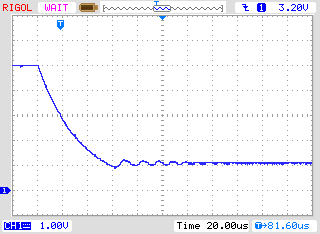
\includegraphics[width=.95\textwidth]{../PNG/AREF2_1V.png}
    \caption{from \(5V\) to \(1.1V\) }
    \label{pic:aref1}
  \end{subfigure}
  ~
  \begin{subfigure}[b]{.5\textwidth}
    \centering
    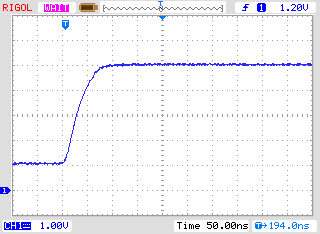
\includegraphics[width=.95\textwidth]{../PNG/AREF2VCC.png}
    \caption{from \(1.1V\) to \(5V\)}
    \label{pic:aref5}
  \end{subfigure}
  \caption{Umschalten von AREF mit einem \(1nF\) Kondensator}
\end{figure}

\begin{description} \setlength{\itemsep}{0em}
  \item[REF\_R\_KORR] gibt einen Offset für die interne Referenz-Spannung in mV-Einheiten an.
Mit diesem Offset kann eine Differenz bei der Umschaltung der Referenzspannung für die Widerstandsmessung abgeglichen werden.
Wenn die AUTO\_CAL-Option gewählt wurde, ist dieser Wert nur ein Offset zu der gefundenen Spannungs-Differenz in der
AUTO\_CAL Funktion.\\
Beispiel: CFLAGS += -DREF\_R\_KORR=10
  \item[OP\_MHZ] gibt der Software an, mit welcher Taktfrequenz in MHz der Tester arbeiten wird.
Die Software ist nur mit \(1MHz\), \(8MHz\) und zusätzlich auch \(16MHz\) getestet. Der Betrieb mit \(8MHz\) wird wegen der besseren Auflösung der
Kondensator- und Spulen-Messung empfohlen.\\
Beispiel: OP\_MHZ = 8
  \item[RESTART\_DELAY\_TICS] muss auf 6 gesetzt werden, wenn der ATmega168 oder ATmega328 ohne Quarz mit dem
RC-Generator betrieben wird. Wenn dieser Wert nicht vorbesetzt wird, wählt die Software die 16384 Takte Startverzögerung für
den Quarzbetrieb.\\
Beispiel: CFLAGS += -DRESTART\_DELAY\_TICS = 6
  \item[USE\_EEPROM] gibt an, ob feste Texte und Tabellen im EEPROM-Speicher abgelegt werden sollen.
Anderenfalls wird der Programmspeicher (Flash) benutzt.
Es wird empfohlen, den EEPROM-Speicher zu benutzen (Option gesetzt).\\
Beispiel: CFLAGS += -DUSE\_EEPROM
  \item[EBC\_STYLE] gibt an, dass die Ausgabe der Transistor-Pinbelegung im Format \inquotes{EBC=...} bzw. \inquotes{GDS=...} erfolgen soll.
  Diese Darstellungsweise spart Programmplatz. Ohne diese Option wird die Belegung im Format \inquotes{123=...} angezeigt, wobei
jeder Punkt ein E (Emitter), B (Basis) oder K (Kollektor) sein kann.
Bei FETs kann jeder Punkt entsprechend ein G (Gate), D (Drain) oder S (Source) sein.
Wenn die Reihenfolge der Testpins nicht 1,2 und 3 in Leserichtung ist, kann die Reihenfolge mit der Option EBC\_STYLE=321 
umgedreht werden. Dann wird die Pinbelegung in der Form \inquotes{321=...}, was der gewohnten Leserichtung von links nach rechts
entgegen kommt, wenn die Testpins die Reihenfolge 3,2,1 haben.\\
Beispiel: CFLAGS += EBC\_STYLE
  \item[NO\_NANO] gibt an, dass der Dezimalpräfix Nano nicht zur Darstellung von Messergebnissen benutzt werden soll.
So werden Kapazitätswerte in \(\mu F\) statt in \(nF\) angegeben.\\
Beispiel: CFLAGS += NO\_NANO
  \item[NO\_LONG\_PINLAYOUT] kann gesetzt werden, um die lange Form der Pinbelegung bei graphischen Displays zu verhindern
wie \inquotes{ Pin  1=E 2=B 3=C}.
Wenn die Option gesetzt ist, wird die kurze Form wie \inquotes{ Pin  123=EBC} benutzt.\\
Example: CFLAGS += NO\_LONG\_PINLAYOUT
  \item[PULLUP\_DISABLE] gibt an, dass man die internen \inquotes{Pull-Up}-Widerstände nicht benötigt.
Sie müssen einen externen \inquotes{Pull-Up} Widerstand an Pin 13 (PD7) und VCC angeschlossen haben, um diese
Option benutzen zu können.
Mit dieser Option wird ein möglicher Einfluss der \inquotes{Pull-Up} Widerstände auf die Mess-Ports (Port B und Port C) verhindert.\\
Beispiel: CFLAGS += -DPULLUP\_DISABLE

  \item[ANZ\_MESS] diese Option gibt an, wie oft der ADC-Wert eingelesen und addiert werden soll.
Sie können einen Wert zwischen 5 und 200 wählen um einen Mittelwert für eine ADC-Messung zu bilden.
Höhere Werte ergeben eine bessere Genauigkeit, aber brauchen längere Messzeit.
Eine ADC-Messung mit dem Wert 44 braucht etwa \(5ms\).\\
Beispiel: CFLAGS += -DANZ\_MESS=44

  \item[POWER\_OFF] Diese Option schaltet die automatische Abschaltfunktion ein.
Wenn Sie diese Option weglassen, werden die Messungen in einer Schleife endlos wiederholt, bis die Betriebsspannung 
unterbrochen wird (Ein/Aus-Schalter).
Wenn Sie einen Tester ohne die Schalttransistoren haben, können Sie diese Option weglassen.

Wenn Sie mit den eingebauten Schalttransistoren die Option POWER\_OFF weggelassen haben,
gibt es dennoch eine Möglichkeit für eine Abschaltung, wenn Sie die WITH\_MENU-Option gewählt haben.

Sie können mit der POWER\_OFF-Option auch angeben, nach wie vielen Messungen ohne gefundenes Bauteil der Tester ausschaltet.
Bei doppelt so viel aufeinanderfolgenden Messungen mit gefundenem Bauteil schaltet der Tester auch ab,
wenn nicht zwischendurch eine Messung ohne gefundenes Bauteil war.
Wenn Sie vergessen haben, ein angeschlossenes Bauteil abzuklemmen, wird so eine vollständige Batterie-Entladung
verhindert.
Bei einer Options-Angabe in der Form von CFLAGS += -DPOWER\_OFF=5 wird nach 5 aufeinanderfolgenden Messungen ohne
gefundenes Bauteil abschaltet. Aufeinanderfolgende 10 Messungen mit gefundenem Bauteil schalten ebenfalls aus.
Nur wenn die jeweilige Mess-Serie durch den anderen Typ unterbrochen wird, wird die Messung fortgesetzt.
Die Messresultate für eine Einzelmessung werden 28~Sekunden angezeigt, bei der Mehrfachmessung wird die
Anzeigezeit auf 5~Sekunden reduziert (wird in config.h gesetzt).
Wenn der Startknopf beim ersten Einschalten lange gedrückt wird, wird das Messergebnis
 auch bei der Mehrfachmessung 28~Sekunden angezeigt.
Der Maximalwert für die Wiederholungen ist 255 (CFLAGS += -DPOWER\_OFF=255).\\
Beispiel 1: CFLAGS += -DPOWER\_OFF=5 \\
Beispiel 2: CFLAGS += -DPOWER\_OFF 

  \item[BAT\_CHECK] schaltet die Batterie-Spannungsprüfung ein.
 Wenn Sie diese Option nicht angeben, wird die Versionsnummer der Software angezeigt.
Diese Option ist hilfreich um bei batteriebetriebenen Tester-Versionen an den Batteriewechsel zu erinnern.\\
Beispiel: CFLAGS += -DBAT\_CHECK

  \item[BAT\_OUT] schaltet die Batterie-Spannungsanzeige auf dem LCD ein, wenn BAT\_CHECK gewählt wurde.
 Wenn Ihre \(9V\)-Versorgung eine Diode als Verpolungsschutz installiert hat, können Sie 
die Form BAT\_OUT=600 angeben, um die Dioden-Schwellspannung 
bei der Spannungsanzeige zu berücksichtigen.
Auch der Spannungsverlust am Transistor T3 kann so mit dieser Option berücksichtigt werden.
Die Angabe der Schwellspannung in mV beeinflusst nicht die Prüf\-span\-nungs Werte (BAT\_POOR).\\
Beispiel 1: CFLAGS += -DBAT\_OUT=300 \\
Beispiel 2: CFLAGS += -DBAT\_OUT

  \item[BAT\_POOR] setzt die Leer-Spannung für die Batteriespannungs-Prüfung auf den angegebenen Wert in Einheiten von \(1mV\).
Die Warn-Spannung ist \(0,8V\) höher als die angegebene Leer-Spannung, wenn die Leer-Spannung mehr als \(5,3V\) beträgt.
Sonst wird eine \(0,4V\) höhere Warn-Spannung gewählt, bei unter \(3,25V\) sogar nur eine \(0,2V\) höhere Warn-Spannung und
bei unter \(1,3V\) nur eine \(0,1V\) höhere Warnspannung als die angegebene Leer-Spannung.
Das Setzen der Leer-Spannung auf Werte wie \(5,4V\) wird für wiederaufladbare \(9V\) Batterien nicht empfohlen,
weil das die Gefahr von Batterie-Schäden aufgrund von Tiefentladung erhöht!
Wenn Sie wiederaufladbare \(9V\)-Batterien einsetzen, werden \inquotes{Ready to Use}-Typen wegen der geringeren Selbstentladung empfohlen.\\
Beispiel für low-drop-Regler (\(5,4V\)): CFLAGS += -DBAT\_POOR=5400 \\
Beispiel für 7805-Regler (\(6,4V\)): CFLAGS += -DBAT\_POOR=6400

  \item[DC\_PWR] Dieser Spannungspegel in mV Einheiten gibt eine Grenze für die Batteriespannung an, oberhalb
  derer der Tester in den \inquotes{DC\_Pwr\_Mode} wechselt. Normalerweise läuft der Tester in einem Batterie-Modus,
wo alle Zusatzfunktionen zeitlich beschränkt laufen.
Mit dem \inquotes{DC\_Pwr\_Mode} laufen die Zusatzfunktionen zeitlich unbeschränkt.
Weil es keinen DC-DC Konverter gibt, der mit einer Eingangsspannung von \(0.9V\) läuft,
wird der \inquotes{DC\_Pwr\_Mode} auch gestartet, wenn eine Batteriespannung unterhalb \(0.9V\) entdeckt wird.\\
Beispiel: CFLAGS += -DDC\_PWR=9500

 \item[BAT\_NUMERATOR] Definiert den Zähler eines Bruchs an, mit dem die Spannung bewertet werden muß,
um die richtige Batteriespannung zu erhalten. Für den Standard-Spannungsteiler mit einem \(10 k\Omega\) und 
einem \(3.3 k\Omega\) Widerstand ist der Quotient (10000 + 3300)/3300. 
Der über die Widerstandswerte erhaltene Quotient sollte gekürzt werden. 
Für das Beispiel ergibt sich 133/33 .\\
Beispiel: CFLAGS += -DBAT\_NUMERATOR=133

 \item[BAT\_DENOMINATOR] Gibt den Nenner eines Bruches an, mit dem die Spannung bewertet werden muß.\\
Beispiel: CFLAGS += -DBAT\_DENOMINATOR=33

 \item[EXT\_NUMERATOR] Definiert den Zähler eines Bruchs an, mit dem die externe Spannung bewertet werden muß,
um die richtige Spannung zu erhalten. Für den Standard-Spannungsteiler mit einem \(180 k\Omega\) und 
einem \(20 k\Omega\) Widerstand ist der Quotient (180000+20000)/20000.
Der Quotient sollte auf 10/1 gekürzt werden.\\
Beispiel: CFLAGS += -DEXT\_NUMERATOR=10

 \item[EXT\_DENOMINATOR] Gibt den Nenner eines Bruches an, mit dem die externe Spannung bewertet werden muß.\\
Beispiel: CFLAGS += -DEXT\_DENOMINATOR=1

  \item[INHIBIT\_SLEEP\_MODE] sperrt die Benutzung des \inquotes{Sleep Mode} (Schlafzustand) des Prozessors.
Normalerweise wird von der Software für längere Pausen der Schlafzustand des Prozessors benutzt, um Strom zu sparen.
Die Benutzung dieses Schlafzustandes mit dem Wiederaufwachen spart zwar Batteriekapazität, 
stellt eine zusätzliche Anforderung für den Spannungsregler dar.\\
Beispiel: DINHIBIT\_SLEEP\_MODE = 1

  \item[PROGRAMMER] \label{sec:config-Prog} stellt den Programmer-Typ für das \lcmd{avrdude} Schnittstellenprogramm ein.\\
Eine richtige Einstellung des Programmer-Typs (und Ports) ist notwendig.\\
In \lname{Makefile} ist standardmäßig Programmer der Firma Diamex eingestellt.\\
Vorbereitet sind aber auch USBasp von Fischler und Arduino Mega.\\
Falls ein anderer Programmer verwendet sein sollte, muss er in \lname{Makefile} aufgenommen werden und der,
bis jetzt aktuelle, mit \#~ am Anfang der Zeile abgewählt werden.\\
Ein Beispiel für die Benutzung von USBtiny Programmer:\\
\# setting for USBtiny ISP\\
PROGRAMMER=usbtiny\\
BitClock=10\\
PORT=usb\\
und ein weiterer Beispiel:\\
\#~setting for Pololu programmer\\
\#~PROGRAMMER=stk500v2\\
\#~BitClock=1.0\\
\#~PORT = /dev/ttyACM0\\
, wenn Sie den \lcmd{make upload}- oder
\lcmd{make fuses}-Aufruf dieser \lname{Makefile} benutzen.
Beispiel: PROGRAMMER=avrisp2

  \item[BitClock] stellt die Bit-Taktperiode für den Programmer ein. Siehe dazu die Beschreibung des -B Parameters von \lcmd{avrdude}.\\
Beispiel: BitClock=5.0

  \item[PORT] stellt die verwendete Schnittstelle ein, wo \lcmd{avrdude} den Mikrocontroller (ATmega) erreichen kann.
  Für weitere Informationen schauen Sie bitte in das Handbuch von \lcmd{avrdude} oder in die Online-Dokumentation~\cite{avrdude}.\\
Beispiel: PORT=usb

\end{description}

Zusätzliche Parameter können in den Dateien Transistortester.h und config.h gesetzt werden.
Die Datei config.h enthält globale Variablen und Tabellen, definiert die Port- / Pin-Konstellation,
die ADC-Taktfrequenz sowie die Widerstandswerte, die für die Messung benutzt werden.
Die Datei Transistortester.h enthält die globalen Variablen und Tabellen sowie die Texte für die LCD-Anzeige.
Normalerweise brauchen diese Werte nicht ohne Grund geändert werden.


\section{Programmierung des Mikrocontrollers}
Ich gebe die Software für den Mikrocontroller in Quelltext heraus.
Die Entwicklung wurde mit dem Linux-Betriebssystem (Ubuntu bzw. Mint) gemacht
und wird gesteuert mit einer \lname{Makefile}.

Die \lname{Makefile} stellt sicher, dass die Software entsprechend der vorher in der \lname{Makefile} 
eingestellten Optionen übersetzt wird. Schauen Sie bitte in die Datei LiesMich.txt
im Verzeichnis default und in das Konfigurations-Kapitel~\ref{sec:config} ab Seite~\pageref{sec:config}.

Das Ergebnis der Übersetzung hat die Dateierweiterung \lname{.hex} und \lname{.eep}.
Die \lname{.hex}-Datei enthält die Daten für den Programmspeicher (Flash) des ATmega-Prozessors.
Die \lname{.eep}-Datei enthält die Daten für den EEPROM des ATmega.\\
Beide Dateien müssen in den richtigen Speicher geladen werden.

Zusätzlich muss der ATmega mit den \inquotes{fuses} richtig konfiguriert werden.\\
Wenn Sie meine \lname{Makefile} zusammen mit dem Programm \lcmd{avrdude} \cite{avrdude} benutzen,
brauchen Sie keine genaue Kenntnis über die Einzelheiten der fuses.

Sie brauchen nur \lcmd{make fuses} aufrufen, wenn Sie keinen Quarz benutzen oder Sie
müssen \lcmd{make fuses-crystal} aufrufen, wenn Sie einen \(8MHz\) Quarz auf der Baugruppe installiert haben.

Bei der ATmega168-Serie der Mikrocontroller können Sie alternativ auch
\lcmd{make fuses-crystal-lp} aufrufen für den low power Quarz-Betrieb.\\
Benutzen Sie niemals die Quarz-Varianten, wenn Sie keinen \(8MHz\) oder \(16MHz\) Quarz installiert haben.

Wenn Sie sich nicht sicher mit den fuses sind, lassen Sie diese erst einmal wie
vom Werk gesetzt und bringen Sie den Tester in diesem Zustand zum Laufen.\\
Es kann sein, dass das Programm zu langsam läuft, wenn Sie die für den \(8MHz\)-Betrieb 
erzeugten Programmdaten benutzen, aber das kann man später korrigieren!
Aber falsch gesetzte fuses können die spätere ISP-Programmierung verhindern.

Vielleicht meldet das Programm \lcmd{avrdude} einen Fehler beim Setzen der extendet Fuse efuse.
Das Lesen von unbenutzten Fuse Bits ist beim ATmega als \inquotes{1} spezifiziert, aber
das \lcmd{avrdude} Programm maskiert die unbenutzten Bits, so daß es eine \inquotes{0} für alle unbenutzen Bits erwartet.
Normalerweise sollte die efuse auf 0xfc gesetzt werden, aber \lcmd{avrdude} liest eine 0x04 mit der Maske zurück.
Man kann die Datei avrdude.conf ändern, um das Verhalten von \lcmd{avrdude} zu ändern oder
die efuse auf 0x04 setzen. 
Alle efuse-Werte können mit dem Bezeichner EFUSE\_VAL am Anfang der Datei setup.mk im Quellcode-Verzeichnis
gesetzt werden. Wahrscheinlich sind die Fuses aber auch mit der Fehlermeldung richtig gesetzt.

\newpage
\subsection{Benutzung von Linux}
\label{sec:linux}

Um meine Erfahrung mit Verzweiflung und \inquotes{schlaflose Nächten} anderen Kollegen zu ersparen,
wurde dieses Unterkapitel geschrieben.
Ich hatte ohne jegliche AVR Erfahrung einen Clonetester erworben und wollte diesem die deutsche Sprache
\inquotes{beibringen}.\\

Die dabei erworbenen Erfahrungen sollen anderen \inquotes{willigen} Unerfahrenen helfen,
ERFOLGREICH ihren Tester zu programmieren.
Diese Gelegenheit wird benutzt, dem Entwickler des Transistortester und Autor dieses Dokuments,  
Karl-Heinz Kübbeler siehe \cite{karlheinz1} zu danken für sein Engagement und Geduld,
denn die folgenden Seiten wären ohne seine Hilfe nie entstanden.
     
Damit das Übersetzen der Firmware und Brennen ins MCU gelingt und gleichzeitig \dots
\inquotes{das Rad nicht neu erfunden werden muss}, wurde ein Teil der folgenden Seiten aus dem
ursprünglichen Original übernommen.

Also noch einmal \dots \LARGE{EINEN RIESEN DANK}
\normalsize an Karl-Heinz Kübbeler.

\subsubsection{Betriebssystem Linux}

Die Programmierung unten Linux bringt viele Vorteile, weil dieses OS von Experten entwickelt wurde,
die sich auf den Wünschen der Benutzer orientieren.
Zudem ist die Umgebung kostenlos erhältlich und perfekt gewartet.
Ein weiterer Vorteil ist die Sicherheit des OS selbst aber auch beim Nutzen des Internets.
Die heutigen Editionen lassen sich noch viel leichter bedienen als die Mitbewerber OS.
Es gibt auch sehr leistungsfähige Editoren wie vim oder emacs, die aber etwas
Einarbeitungszeit erfordern. Speziell vim hat den Vorteil, daß er praktisch auf
jedem System vorinstalliert ist. Aber gerade bei diesem Editor ist der
Wechsel zwischen Eingabe-Modus und Befehls-Modus gewöhnungsbedürfig.
Diese Anleitung soll alle \inquotes{nicht} Linux Benutzer dazu animieren es NUN zu testen
indem sie ihr Tester damit programmieren.

Die nachfolgenden Beispiele wurden mit Linux Mint getestet, das
mit drei verschiedenen Desktop Umgebungen angeboten wird (cinnemon, MATE und Xfce).
Die nachfolgenden Hinweise sollten aber bei allen drei Desktops funktionieren.
Die Installation ist auf verschiedene Arten möglich und bringt seinen eigenen Bootmanager mit,
damit man sein vorhandenes OS weiter parallel nutzen kann.

\subsubsection{Tipps für die Linux Nutzung}

Zuerst möchte ich einen Hinweis geben für alle, die nicht gerne Texte abschreiben.
Sie können dieses Handbuch auf einen USB-Stick kopieren und im Dateibrowser mit Doppelclick der
linken Maustaste \LMB öffnen.
Alternativ zum Doppelklick kann mit der \RMB Taste ein anderes als das
vorgewählte PDF Betrachtungsprogramm ausgewählt werden.
Das geöffnete Fenster kann auf dem Bildschirm verschoben werden und auch in der Größe
angepasst werden. Dazu gibt es in der Regel verschiedene Möglichkeiten.
Eine davon ist die \RMB Taste zu drücken, wenn der Mauszeiger 
auf die Kopfzeile des Fensters zeigt und dann die Funktion \menu[,]{Verschieben} auszuwählen.
So kann man das Fenster mit der PDF-Dokumentation beispielsweise an die linke Bildschirmseite
verschieben. Durch Drücken der linken Maustaste rastet das Fenster an der neuen Position ein.
Zum Verschieben kann man auch mit der \LMB Taste die
Kopfleiste des Fensters packen und bei weiter gedrückter \LMB Taste verschieben.
Dann rastet das Fenster auf der Position ein, wenn man die Maustaste loslässt.

Im nächsten Schritt wird die Tastenkombination \keys{{Strg} + \Alt + T} gleichzeitig gedrückt,
um ein (neues) Befehlsfenster zu öffnen.
Dies wird nun auf die schon beschriebene Weise zur rechten Hälfte des Bildschirmes verschoben und
kann auch in der Größe verändert werden.
Die Größenänderung kann mit der \LMB Taste an den Rändern oder Ecken des Fenstern gemacht werden,
oder auch mit der \RMB Taste an der Kopfleiste mit der \menu[,]{{Größe ändern}} Funktion.
Die Bedienung ist sonst gleich wie beim Verschieben.\\

In der Regel besitzen die graphischen Oberflächen bei Linux mehr als eine Arbeitsfläche,
die mit der Tastenkombination \keys{{Strg} + \Alt + \arrowkeyright}
beziehungsweise \keys{{Strg} + \Alt + \arrowkeyleft} umgeschaltet werden können.
Mit der \RMB Taste können Sie auf der Kopfzeile der Fenster eine
der Arbeitsflächen wählen, auf der das Fenster angezeigt wird.

So kann man die für die Arbeit benötigten Fenster auf einer Arbeitfläche
zusammen sammeln und erstickt nicht in all den Fenstern für verschiedene Arbeitsbereiche. 
Bei allen Befehlseingaben und Dateibezeichnern ist übrigens darauf zu  achten,
daß bei Linux zwischen Groß und Kleinschreibung unterschieden wird.


\subsubsection{Programm Pakete installieren}

Zum Installieren von Software-Paketen braucht ihr Rechner einen Internetzugang.
Bevor Sie den Tester programmieren konnen, müssen zuerst die Programmpakete
binutils-avr, avrdude, avr-libc und gcc-avr installiert werden.
Jetzt können sie den unten angegebenen Befehl durch Abtippen
mit der Tastatur ausführen lassen.
Sie können aber auch im geöffneten PDF Dokument an diese Stelle blättern
und den nachfolgenden Text mit der gedückten linken Maustaste \LMB markieren:
\begin{large} \vspace{-0.4em} \begin{verbatim}
sudo apt-get install avrdude avr-libc binutils-avr gcc-avr git
\end{verbatim} \end{large}
Am Ende des Textes muß die Maustaste \LMB losgelassen werden,
um die Markierung abzuschließen.
wenn der Text in einer eigenen Zeile steht, wie in diesem Beispiel, können
die den Text auch mit dreimaligem \LMB Maus Click irgendwo auf der Zeile markieren.
Danach kann man den Mauszeiger in das rechte Befehlsfenster führen und
durch Drücken der mittlerer Maustaste {weiter als \MMB abgekürzt} den vorhin
markierten Text in die Befehlszeile einfügen.
Bei vielen Mäusen ist das Scoll-Rad gleichzeitig die mittlere Maustaste.
Bei Mäusen ohne mittlere Maustaste ist es möglich die mittlere Maustaste
durch gleichzeitiges Drücken der \LRMB Maustasten zu ersetzen.
Egal, wie der Befehlstext nun in die Befehlszeile gekommen ist,
sie sollten den Text noch einmal kontrollieren, bevor
sie den Befehl durch Dücken der \keys{\enter} Taste abschicken.
In der Regel brauchen Sie keine Angst zu haben, daß durch die Installation
von Paketen etwas schlimmes durch Fehlbedienung passiert.
Das Programm \lcmd{apt-get} prüft vor dem Ausführen der Operation, ob die aufgeführten
Pakete schon installiert sind und die Abhängigkeiten erfüllt sind.
Gegebenenfalls wird aber ein schon vorher installiertes Paket durch ein neueres ersetzt.
Dann wird das \lcmd{sudo} Programm Sie zunächst nach den Benutzer Passwort fragen,
bevor es den Rest der Befehlszeile ausführt.
Sie sollten das Passwort mit Drücken der \keys{\enter} oder \keys{\return} Taste abschließen und bestätigen.
Damit werden nun alle Software Pakete durch \lcmd{apt-get} herunter geladen und installiert.\\

Es kann sein, daß \lcmd{apt-get} bei der Installation der Pakete Fragen stellt,
die man in der Regel mit der Taste \keys{J} beantworten kann.

Natürlich gibt es auch andere Wege, die Pakete zu installieren, welche eine graphische Oberfläche benutzen
wie \lcmd{synaptic} oder \lcmd{dpkg}. Aber es nicht einfacher eine gemischte Gruppe von Paketen anzugeben.
Wenn sie irgendeine dieser Paketmanager, sollten sie über alle installierten Pakete Bescheid wissen,
egal auf welchem Wege sie installiert wurden.
Die graphischen Paketmanager können auch dabei helfen, den Namen der Pakete herauszufinden.

\subsubsection{Download der Quellen}

Ob die Versionsverwaltung \lcmd{git} erfolgreich installiert wurde,
kann man mit dem folgenden Kommando prüfen:
\begin{large} \vspace{-0.4em} \begin{verbatim}
git version
\end{verbatim} \end{large}
Das \lcmd{git} Programm sollte mit der Ausgabe seiner Versionsnummer antworten.
Falls in Ihrem Heimatverzeichnis schon ein Ordner TransistorTester-source existiert,
sollte man den umbenennen oder löschen.
Das Programm \lcmd{git} wird für den Download der Quellen und Dokumentation benutzt.
Mit dem Befehl:
\begin{large} \vspace{-0.4em} \begin{verbatim}
git clone https://github.com/kubi48/TransistorTester-source
\end{verbatim} \end{large}
wird das aktuelle Transistortester Quellcode-Archiv heruntergeladen.
Die Dateien sind nun in dem Linux [Persönlicher Ordner] , üblicherweise \lname{/home/} gefolgt
von Ihrem Benutzerkürzel, mit dem  Verzeichnisnamen \lname{TransistorTester-source}.
Mit der Terminaleingabe  \lcmd{ls} \(\mbox{\keys{l} \keys{s} \keys{\return}}\) kann man
das Vorhandensein überprüfen.
Mehr Informationen über Dateien und Verzeichnisse erhält man mit
dem Kommando \lcmd{ls -lh}. Hier wurden jetzt zwei Optionen für das Kommando \lcmd{ls} zusammengefasst,
die \lcmd{{ -l}} Option und die \lcmd{{ -h}} Option. Diese Eingabeform ist also eine Kurzform für
das Kommando \lcmd{ls -l -h} oder auch \lcmd{ls -l {-}{-}human-readable}.
Einige der Optionen sind in zwei Versionen vorhanden, einer kurzen mit einem - (\lcmd{{ -h}})
und einer langen Form mit zwei - (\lcmd{{ {-}{-}human-readable}}).
Die Reihenfolge der Optionen spielt übrigens keine Rolle,
genau wie die Anzahl der trennenden Leerzeichen \keys{\space}.
Bei fast allen Kommandos erfährt man mehr über die Bedienung und die Optionen
durch durch Anhängen der \lcmd{{ --help}} Option.
Das gilt natürlich auch für das Kommando \lcmd{git}.\\

Um neue Updates heruntergeladen, reicht es in der Zukunft, 
\begin{large} \vspace{-0.4em} \begin{verbatim}
git pull
\end{verbatim} \end{large}
im Arbeitsverzeichnis \lname{TransistorTester-source} einzugeben.
Das kann je nach Kommandointerpreter auch mit
\begin{large} \vspace{-0.4em} \begin{verbatim}
(cd ~/TransistorTester-source ; git pull)
\end{verbatim} \end{large}
aus jedem Arbeisverzeichnis erfolgen.
Damit der \lcmd{git pull} einwandfrei funktioniert, sollte man den
Verzeichnisbaum besser nicht verändern.

\subsubsection{Übersetzen der Transistortester Quellen}

Zum Übersetzen der Transistortester-Quellen ist nur ein \lcmd{make} Aufruf
im richtigen Arbeitsverzeichnis erforderlich.
Da aber auch mit \lcmd{make upload} der ATmega mit einem angeschlossenen
ISP-Programmer programmiert werden kann, ist es sinnvoll,
sich zunächst mit den Schnittstellen für den Anschluß des ISP-Programmer
zu beschäftigen.
Der weitere Arbeitsablauf ist dann unter Punkt \ref{sec:Arbeitsumgebung} auf
Seite \pageref{sec:Arbeitsumgebung} beschrieben.

\subsubsection{Benutzung der Schnittstellen}
\label{sec:Schnittstellen}

Alle modernen ISP-Programmer mit serieller Schnittstelle benutzen gerne die USB Schnittstelle,
da diese Schnittstelle auch gleich die Stromversorgung sicherstellt.
Für diese Geräte sollten Sie überprüfen, welche Gerätebezeichnung
diesem Gerät zugeordnet ist.
Beim Einstecken eines USB Gerätes wird bei Linux ein Eintrag in das
Systemprotokoll vorgenommen.
Da das Systemprotokoll eine Textdatei ist,
kann man diese einfach auf dem Bildschirm anzeigen.
Dazu kann man in Konsolfenster den Befehl dmesg benutzen und da wir nach dem
Einstecken des Programmers nur an den letzten Zeilen des Protokolls
interessiert sind, benutzt man:
\begin{large} \vspace{-0.4em} \begin{verbatim}
dmesg|tail
\end{verbatim} \end{large}
Das \lcmd{dmesg} Programm zeigt das gesamte Systemprotokoll und das Kommando 
\lcmd{tail} zeigt nur die letzten 10 Zeilen der Ausgabe.
Für einen Pololu Programmer sieht das Ergebnis so aus:
\begin{footnotesize} \begin{verbatim}
usb 1-3: new full-speed USB device number 3 using xhci_hcd
usb 1-3: New USB device found, idVendor=1ffb, idProduct=00bb, bcdDevice= 1.02
usb 1-3: New USB device strings: Mfr=1, Product=2, SerialNumber=3
usb 1-3: Product: Pololu USB AVR Programmer v2.1
usb 1-3: Manufacturer: Pololu Corporation
usb 1-3: SerialNumber: 00227484
cdc_acm 1-3:1.1: ttyACM0: USB ACM device
cdc_acm 1-3:1.3: ttyACM1: USB ACM device
usbcore: registered new interface driver cdc_acm
cdc_acm: USB Abstract Control Model driver for USB modems and ISDN adapters
\end{verbatim} \end{footnotesize}
Wichtig sind hier die Zeilen 7 und 8 mit den Einträgen ttyACM0 und ttyACM1.
Das sind die zugewiesenen Gerätebezeichnungen für zwei serielle Schnittstellen.
Bei Linux sind alle Geräte auch Bestandteil des Dateibaums und im
Ordner \lname{/dev/} eingetragen. Mit vollständigem Namen heißen die
beiden seriellen Schnittstellen also \lname{/dev/ttyACM0} und \lname{/dev/ttyACM1}.
Für den Pololu Programmer muß man wissen, daß die erste serielle Schnittstelle
für den ISP-Programmer benutzt wird und die zweite serielle Schnittstelle
für andere Zwecke frei benutzt werden kann.
Sie können die Existenz der Geräteeintragungen mit dem Kommando
\begin{large} \vspace{-0.4em} \begin{verbatim}
ls -l /dev/ttyACM*
\end{verbatim} \end{large}
überprüfen. Das Ergebnis sollte dann so aussehen:
\begin{footnotesize} \begin{verbatim}
crw-rw---- 1 root dialout 166, 0 Mär 11 09:57 /dev/ttyACM0
crw-rw---- 1 root dialout 166, 1 Mär 11 09:57 /dev/ttyACM1
\end{verbatim} \end{footnotesize}
Bei dieser Ausgabe kann man lesen, daß der Zugriff für den Benutzer \lname{root}
und für die Benutzergruppe \lname{dialout} erlaubt ist.
Mit dem Kommando \lcmd{id} können Sie ihre Gruppenzugehörigkeit überprüfen.
Hier sollte die Gruppe \lname{dialout} in der Liste auftauchen,
sonst wird im nächsten Arbeitspunkt die Änderung der Gruppenzugehörigkeit
beschrieben.
Ein anderes Beispiel für das Systemprotokoll eines anderen
ISP-Programmers \inquotes{Diamex ISP-PRog NG} sehen sie hier:
\begin{footnotesize} \begin{verbatim}
usb 1-6: new full-speed USB device number 8 using xhci_hcd
usb 1-6: New USB device found, idVendor=16c0, idProduct=2a9b, bcdDevice=43.40
usb 1-6: New USB device strings: Mfr=1, Product=2, SerialNumber=3
usb 1-6: Product: AVR-ISP2
usb 1-6: Manufacturer: ERFOS
usb 1-6: SerialNumber: 19377-43111-757
cdc_acm 1-6:1.0: ttyACM0: USB ACM device
\end{verbatim} \end{footnotesize}

Bei diesem Beispiel ist der Gerätename identisch (ttyACM0).\\

Einen Überblick über die angeschlossenen USB-seriell Wandler geben auch
die Eintragungen in Verzeichnis \lname{/dev/serial/by-id/},
die man mit dem Kommando abfragen kann:
\begin{large} \vspace{-0.4em} \begin{verbatim}
ls -og /dev/serial/by-id/* | cut -d' ' -f 7-
\end{verbatim} \end{large}
Die Ausgabe kann beispielsweise so aussehen:
\begin{footnotesize} \begin{verbatim}
/dev/serial/by-id/usb-Arduino__www.arduino.cc__0043_954323131383519062F0-if00 -> ../../ttyACM2
/dev/serial/by-id/usb-Pololu_Corporation_Pololu_USB_AVR_Programmer_v2.1_00227484-if01 -> ../../ttyACM0
/dev/serial/by-id/usb-Pololu_Corporation_Pololu_USB_AVR_Programmer_v2.1_00227484-if03 -> ../../ttyACM1
\end{verbatim} \end{footnotesize}
Wenn die Beschreibung ausführlich genug ist, kann man so die Schnittstellen zuordnen.


Wenn bis zu diesem Schritt alles in Ordnung ist,
muß für dieses Beispiel nur der PORT Eintrag in der \lname{Makefile} auf
\inquotes{PORT=/dev/ttyACM0} geändert werden,
damit das \lcmd{avrdude} Programm auf den Programmer zugreifen kann.
Wenn bei Ihrem System noch andere USB-seriell Schnittstellen benutzt
werden, können die letzten Ziffern der Gerätebezeichnung abweichen.
Erwähnen möchte ich auch, daß eine andere Gruppe von USB-seriell
Schnittstellen statt ttyACM den Namen ttyUSB verwendet.\\

Wenn Ihr Programmer eine spezielle USB-Schnittstelle benutzt und
keinen USB-seriell Typ, ist wahrscheinlich noch zusätzliche
Arbeit erforderlich. Als PORT kann hier fest \inquotes{usb} in der \lname{Makefile}
eingetragen werden. Es ist aber wahrscheinlich, daß Sie trotzdem
keinen Zugriff auf das Gerät haben.
Alle angeschlossenen USB-Geräte können durch Eingabe von \lcmd{lsusb} im Befehlsfenster 
angezeigt werden.
Geben Sie \lcmd{lsusb} zuerst ohne und dann mit angeschlossenem USB-Programmer ein.
Ein Vergleich der Ergebnisse lokalisiert den USB-Programmer.

Das Ergebnis von \lcmd{lsusb} kann so aussehen:
\begin{footnotesize} \begin{verbatim}
Bus 001 Device 001: ID 1d6b:0002 Linux Foundation 2.0 root hub
Bus 002 Device 003: ID 046d:c050 Logitech, Inc. RX 250 Optical Mouse
Bus 002 Device 058: ID 03eb:2104 Atmel Corp. AVR ISP mkII
Bus 002 Device 059: ID 2341:0042 Arduino SA Mega 2560 R3 (CDC ACM)
Bus 002 Device 001: ID 1d6b:0001 Linux Foundation 1.1 root hub}
\end{verbatim} \end{footnotesize}
Hier wurde als Device 58 ein AVR ISP mkII erkannt (DIAMEX ALL-AVR).
Das ebenfalls entdeckte Gerät mit der Nummer 59 gehört zur Gruppe der \inquotes{USB-seriell} Geräte.
Die ID 03eb ist eine Herstellerkennung und die ID 2104 eine Produktkennung für diesen ISP-Programmer.
Diese beiden Kennungen werden der Datei /etc/udev/rules.d/90-atmel.rules benötigt und erstellt
mit Hilfe von:
\begin{large} \vspace{-0.4em} \begin{verbatim}
sudo xed /etc/udev/rules.d/90-atmel.rules
\end{verbatim} \end{large}
Natürlich können Sie auch einen anderen Editor als xed benutzen, wenn Sie möchten.
In diesem Beispiel besteht die Datei 90-atmel.rules aus einer Zeile:
\begin{footnotesize} \vspace{-0.4em} \begin{verbatim}
SUBSYSTEM=="usb", ATTRS{idVendor}=="03eb", ATTRS{idProduct}=="2104", MODE="0660", GROUP="plugdev"
\end{verbatim} \end{footnotesize}
Dieser Eintrag erlaubt den Zugriff auf das Gerät für Mitglieder der Gruppe \lname{plugdev}.
Man kann den Eintrag auch ohne Editor direkt mit einem Kommando erzeugen:
\begin{footnotesize} \vspace{-0.4em} \begin{verbatim}
sudo echo 'SUBSYSTEM=="usb", ATTRS{idVendor}=="03eb", ATTRS{idProduct}=="2104"
, MODE="0660", GROUP="plugdev"' >> /etc/udev/rules.d/90-atmel.rules
\end{verbatim} \end{footnotesize}
Die beiden Zeilen müssen sie zu einer langen Zeile 
in der Kommandozeile zusammenfügen!
\newline
Um die meisten Programmer verwenden zu können, wird folgender Text in 90-atmel.rules empfohlen:
\begin{tiny}
\begin{verbatim}
# Copy this file to /etc/udev/rules.d/90-atmel.rules
# AVR ISP mkII - DIAMEX ALL-AVR
SUBSYSTEM=="usb", ATTRS {idVendor}=="03eb", ATTRS {idProduct}=="2104", GROUP = "plugdev", MODE="0660",
# Atmel AVR Dragon
ATTRS {idVendor}=="03eb", ATTRS {idProduct}=="2107", GROUP="plugdev", MODE="0660"
# Atmel-ICE
SUBSYSTEM=="usb", ATTRS {idVendor}=="03eb", ATTRS {idProduct}=="2141", GROUP = "plugdev", MODE="0660",
# xplained-mini
SUBSYSTEM=="usb", ATTRS {idVendor}=="03eb", ATTRS {idProduct}=="2145", GROUP = "plugdev", MODE="0660",
# avrftdi
#SUBSYSTEM=="usb", ATTRS {idVendor}=="0403, ATTRS {idProduct}=="6010", GROUP = "plugdev", MODE="0660",
# UM232H
#SUBSYSTEM=="usb", ATTRS {idVendor}=="0403, ATTRS {idProduct}=="6014", GROUP = "plugdev", MODE="0660",
# USB asp programmer
ATTRS {idVendor}=="16c0", ATTRS {idProduct}=="05dc", GROUP="plugdev", MODE="0660"
# USB NIBObee-Programmer
ATTRS {idVendor}=="16c0", ATTRS {idProduct}=="092f", GROUP="plugdev", MODE="0660"
# USBtiny programmer
ATTRS {idVendor}=="1781", ATTRS {idProduct}=="0c9f", GROUP="plugdev", MODE="0660"
# USB ISP-programmer für Atmel AVR
SUBSYSTEM=="usb", ENV {DEVTYPE}=="usb_device", SYSFS {idVendor}=="16c0", SYSFS {idProduct} == "05dc", MODE="0660",
\end{verbatim}
\end{tiny}
\vspace*{-.8em}
Nach dem die Datei erstellt wurde, kann die Erstellung und Inhalt kontrollieren mit:
\begin{large} \vspace{-0.4em} \begin{verbatim}
less /etc/udev/rules.d/90-atmel.rules 
\end{verbatim} \end{large}
Danach sollten Sie das System veranlassen, die udev-Regeln neu einzulesen mit:
\begin{large} \vspace{-0.4em} \begin{verbatim}
sudo udevadm control --reload-rules
\end{verbatim} \end{large}
Dann sollten Sie den ISP-Programmer ausstecken und wieder einstecken.
Jetzt sollte das System Ihnen Zugriff auf das Gerät geben, wenn Sie Mitglied der Gruppe \lname{plugdev}
sind.
Daher sollten Sie Mitglied der Gruppe \lname{plugdev} und auch der Gruppe \lname{dialout}
sein, damit Sie beide ISP-Programmertypen nutzen können.

\subsubsection{Gruppen Mitgliedschaft}

Deswegen sollte die eigene Benutzerkennung sowohl Mitglied der Gruppe \lname{plugdev} als auch
der Gruppe \lname{dialout} sein. Das Kommando:
\begin{large} \vspace{-0.4em} \begin{verbatim}
sudo usermod -a -G dialout,plugdev $USER
\end{verbatim} \end{large}
sollte die Zugehörigkeit sicherstellen. 
Kontrollieren kann man es mit dem Kommando: \lcmd{id}. 
Wenn die Gruppenmitgliedschaft richtig gemeldet wird,
sollte jetzt ein Zugriff mit \lcmd{avrdude} auf ISP-Programmer mit beiden Schnittstellentypen möglich sein.

Mann kann sich die Gruppenmitgliedschaft auch mit einem Programm mit graphischer Bedienoberfläche ansehen:
\menu[,]{Menü,Systemverwaltung,{Benutzer und Gruppen},{?Passwort}}.
Das \menu[,]{Menü} kann man auch mit der \keys{\winmenu} Taste (zwischen \keys{{Strg}} und
\keys{\Alt}) öffnen.
Aber das Layout der Funktion ist unterschiedlich je nach Desktop Umgebung.

\subsubsection{Arbeitsumgebung und Übersetzen der Quellen}
\label{sec:Arbeitsumgebung}
Damit das Original erhalten bleibt,
wird empfohlen, ein Duplikat der Quellen mit Namen \textbf {Mytester} anzulegen.
Üblicherweise heißt das Home-Verzeichnis \lname{/home/} gefolgt von ihrem Benutzerkürzel.
Der Name ihres Home-Verzeichnisses ist in der System-Variablen \lname{\$HOME} abgelegt.
Sie können statt des Namens in Befehlen auch kurz \lname{\textasciitilde/} schreiben.
Vergessen sie nicht den \lname{/} nach dem \lname{\textasciitilde} Zeichen, sonst würde der
Kommandointerpreter nach einem Benutzer mit dem nachfolgenden Namen suchen!
Dazu legen Sie erst einmal ein leeres Verzeichnis an mit:
\begin{large} \vspace{-0.4em} \begin{verbatim}
mkdir ~/Mytester
\end{verbatim} \end{large}
 \vspace{-0.5em} 
Wenn Sie den Download vom Archiv in das Verzeichnis \lname{\textasciitilde/TransistorTester-source}  durchgeführt haben,
können Sie den nachfolgenden Befehl ausführen, um die Quelldateien und dessen Unterverzeichnisse
in das Mytester Verzeichnis zu kopieren.
\begin{large} \vspace{-0.4em} \begin{verbatim}
rsync -auv ~/TransistorTester-source/trunk ./Mytester
\end{verbatim} \end{large}
 \vspace{-0.5em} 
Wegen der \lcmd{-v} Option protokolliert \lcmd{rsync} alle Kopiervorgänge.
Wenn Sie statt der \lcmd{-auv} Optionen also \lcmd{-au} als Optionen angeben,
bleibt der Kopiervorgang stumm.
Sie können sich aber vom gefüllten Unterverzeichnis mit folgendem Befehl
überzeugen:
\begin{large} \vspace{-0.4em} \begin{verbatim}
ls -lh ~/Mytester/trunk
\end{verbatim} \end{large}
 \vspace{-0.5em} 
Eine übersichtliche Darstellung der Verzeichnisstruktur und der Dateien ist mit dem Kommando
\begin{large} \vspace{-0.4em} \begin{verbatim}
tree ~/Mytester
\end{verbatim} \end{large}
 \vspace{-0.5em} 
möglich. Das Kommando ist aber nicht als Standard installiert, was sie aber mit
\begin{large} \vspace{-0.4em} \begin{verbatim}
sudo apt-get install tree
\end{verbatim} \end{large}
 \vspace{-0.5em} 
leicht nachholen können.\\
Wenn Sie jetzt wissen, welches Unterverzeichnis für Ihren Tester paßt,
können Sie in dieses Unterverzeichnis wechseln.
Nehmen wir mal an, Sie besäßen einen chinesischen Bausatz mit SW-Display, 
dann wäre das Unterverzeichnis \lname{mega328\_st7565\_kit} richtig.
Der Befehl dazu wäre dann:
\begin{large} \vspace{-0.4em} \begin{verbatim}
cd ~/Mytester/mega328_st7565_kit
\end{verbatim} \end{large}
\vspace{-0.5em} 
Mit einem simplen \lcmd{make} Aufruf würde der Quellcode mit
den voreingestellen Einstellungen in der \lname{Makefile} neu übersetzt.

\subsubsection{Methode mit grafische Oberfläche}
Wenn das MyTester Verzeichnis schon angelegt ist, können Sie auch mit
dem Dateien Fenster in das gewünschte Verzeichnis wechseln.
Sie können die Dateien in \lname{\textasciitilde/Mytester/} auch mit dem Dateien Fenster ansehen
\menu[,]{Menü, Zubehör, Dateien}, dabei muß das Verzeichnis \lname{Mytester} durch \LMB Doppelclick ausgewählt werden.
Hier erscheinen jetzt viele Unterverzeichnisse, darunter auch beispielsweise
\lname{mega328\_st7565\_kit}.
Wenn Sie dieses jetzt auch dieses Verzeichnis mit \LMB Doppelclick auswählen,
sehen Sie unter den Files auch die \lname{Makefile}.
Wenn Sie das geschafft haben, können sie jetzt mit der \RMB Taste die Funktion \menu{Im Terminal öffnen}
auswählen und schon öffnet sich ein Kommandofenster mit dem richtigen Arbeitsverzeichnis,
welches auch direkt aktiv ist. Jetzt brauchen sie nur noch \lcmd{make} einzutippen und schon wird
das Transistortester Programm neu übersetzt.
Sie haben jetzt zwei Fenster, die schon auf dem richtigen Arbeitsverzeichnis stehen.
Das Dateien-Fenster und das Terminal-Fenster für die Befehls-Eingabe \lcmd{make}.

\subsubsection{Bearbeitung von Makefile}
Durch \LMB Doppelclick auf die \lname{Makefile} Datei im Dateien-Fenster öffnet sich ein weiteres Fenster
mit dem voreingestellten Editor. Wenn Sie hier einen anderen Editor bevorzugen, können Sie
diesen Editor entweder direkt über \RMB \menu[,]{{Öffnen mit}} auswählen.
Wenn Sie immer einen anderen Editor für Text-Dateien einstellen möchten,
ist das ebenfalls über \RMB  \menu[,]{Eigenschaften} möglich.
Dann öffnet sich ein neues \verb"Eigenschaften von Makefile" Fenster, wo sie die
Funktion \menu[,]{{Öffnen Mit}} durch \RMB anklicken auswählen können.
Hier sehen sie jetzt die aktuelle Einstellung und eine Auswahl an Möglichkeiten zum Bearbeiten
der \lname{Makefile}. Hier können Sie durch \LMB anklicken eine andere Anwendung auswählen.
Durch \LMB Anklicken können sie jetzt auswählen, ob sie diese Anwendung \menu[,]{{Zur Liste hinzufügen}}
oder \menu[,]{{Als Vorgabe festlegen}} möchten.
Sie können die Einstellung aber auch wieder \menu[,]{{Auf Systemvorgabe zurücksetzen}}.
Für den nächsten Schritt ist es wichtig, daß die Einstellungen für
\textbf{ihren ISP-Programmer} in der \lname{Makefile} richtig eingestellt sind.
Siehe dazu im Unterkapitel \ref{sec:config}, auf der Seite \pageref{sec:config-Prog},
Thema \textbf{PROGRAMMER} und \textbf{PORT}.
Nach dem sie diese Einstellungen überprüft haben, speichern sie die Makefile.
Vor dem Eintippen eines Kommandos muß das Terminal-Fenster durch einen \LMB Klick
aktiviert werden. Ein aktiviertes Fenster wird durch einen höheren Kontrast in der
Kopfzeile angezeigt.
Sie haben jetzt zwei Fenster, die schon auf dem richtigen Arbeitsverzeichnis stehen.
Das Dateien-Fenster und das Terminal-Fenster für die Befehls-Eingabe \lcmd{make}.
Natürlich läßt sich ein Editor zum Bearbeiten der \lname{Makefile} auch direkt
aus dem Terminal-Fenster aufrufen. Dann wäre das Dateienfenster nicht erforderlich.


Endlich ist es so weit:
\subsubsection{Tester programmieren}
Wenn Sie das geschafft haben, und ihr ISP-Programmer komplett angeschlossen ist, also eine Verbindung
zum Rechner und zum ATmega hat, brauchen sie nur das Kommando eingeben:
\begin{large} \vspace{-0.4em} \begin{verbatim}
make upload
\end{verbatim} \end{large}
Das Transistortester Programm wird jetzt noch einmal neu übersetzt und dann sofort
mit dem Programm \lcmd{avrdude} in den ATmega geladen.
Falls der Erfolg nicht so aussieht, wie soll, können sie nun sofort zum \lname{Makefile} Editor wechseln,
nötige Änderungen machen und den Prozess wiederholen.

\subsubsection{Tipps zum Terminal} 
Sie brauchen die Befehle nicht jedes mal neu eintippen.
Bereits abgegebene Befehle in dem Terminal Fenster lassen sich mit der \keys{$\uparrow$} Taste
wieder anzeigen.
Den angezeigten Befehl können sie durch Drücken der \keys{\enter} oder \keys{\return}
Taste wiederholen.
Sie können aber auch der angezeigten Befehl vor dem Abschicken editieren,
oder mit der \keys{$\downarrow$} wieder zu neueren Befehlen wechseln.\\

\subsubsection{Mögliche Makefile Aufrufe} 
Zum Schluß sind hier noch einmal die wichtigsten \lname{Makefile} Aufrufe aufgelistet:

\begin{table}[H]
%  \begin{center}
    \begin{tabular}{ l | l}
    Befehl     & Bedeutung\\
    \hline
\lcmd{make clean} 		& zum reinigen des Arbeitsumgebung\\
\lcmd{make}      		& zum Übersetzen des Programms\\
    \lcmd{make fuses}		& zum setzen von ATmega \inquotes{fuses} ohne Quarz\\
    \lcmd{make fuses-crystal}	& zum Setzen von ATmega \inquotes{fuses} NUR mit Version mit Quarz!\\
\lcmd{make upload}		& zum Laden des kompletten Programms über die ISP Schnittstelle in den ATmega.\\
    \end{tabular}
%  \end{center}
%  \caption{}
%  \label{}
\end{table}

\subsubsection{Hinweise zum Update der Transistortester-Quellen}
Die Kopie der transistortester-Quellen kann mit dem Kommando
\begin{large} \vspace{-0.4em} \begin{verbatim}
(cd ~/TransistorTester-source ; git pull)
\end{verbatim} \end{large}
auf dem aktuellen Stand gehalten werden.
Wenn man wie hier empfohlen in einer Kopie unter \lname{\textasciitilde/Mytester} arbeitet,
werden die Änderungen erst übertragen, wenn man auch das Kommando
\begin{large} \vspace{-0.4em} \begin{verbatim}
rsync -auv ~/TransistorTester-source/trunk ~/Mytester
\end{verbatim} \end{large}
ausführt.
Dabei kann es passieren, daß die \lname{Makefile} auf dem github Server ein neueres Datum 
hat als die hier lokal geänderte Kopie. Dann würden die hier lokal im Mytester Ordner
durchgeführten Änderungen der Optionen in der \lname{Makefile} verlorengehen.
Daher ist es eine gute Idee, die erfolgreich geänderte \lname{Makefile} als Kopie
zu sichern. Das kann beispielsweise mit dem Befehl \lcmd{cp Makefile Makefile.bak}
erfolgen. Dann kann man mit dem Befehl \lcmd{diff Makefile Makefile.bak}
die Dateien nach einem Update vom Rechner vergleichen lassen.
Ein besserer Überblick der Änderungen ist auch mit \lcmd{kdiff3 Makefile Makefile.bak}
möglich. Das Programm muß aber wahrscheinlich mit \lcmd{sudo apt-get install kdiff3}
erst installiert werden, da es eigentlich für die KDE Desktopumgebung entwickelt wurde.

\newpage
\subsection{Erstellen der Software unter Windows}
Wahrscheinlich ist derzeit der einfachste Weg, zuerst die Arduino IDE (Integrierte Entwicklungsumgebung) zu installieren.
Dieses Softwarepaket installiert eine aktuelle Version des avr-gcc Kompilers, der dann
auch außerhalb der IDE benutzbar ist, weil der Pfad zu den Programmen in der PATH Variablen von Windows eingetragen ist.
Normalerweise werden die Programme in C:\textbackslash Arduino\textbackslash hardware\textbackslash tools\textbackslash avr\textbackslash bin installiert.
Dort ist dann auch das avrdude Programm für die Bedienung des IDE-Programmers zu finden.
Lediglich ein GNU make Programm fehlt, um die Makefile nutzen zu können.
Dieses Programm habe ich mit dem Cygwin64 Paket installiert.
Für den Download der Transistortester Software wird das Programm git benutzt,
das ebenfalls im Cygwin64 Paket vorhanden ist und sich bei der Installation auswählen läßt.
Das Cygwin64 Paket benutzt einen eigenen Installer setup-x86\_64.exe, der sowohl für Neuinstallationen oder Updates als
auch für Nachinstallation fehlender Tools benutzt wird.
Das ehemals gesamte Transistortester Archiv ist jetzt aufgeteilt in drei verschiedene github Archive.
Die Dokumentation und Quellen alter Versionen befindet sich auf http://github.com/kubi48/TransistorTester-old-versions .
Die aktuelle Dokumentation findet man unter http://github.com/kubi48/TransistorTester-documentation .
Die letzten Quellen findet man unter http://github.com/kubi48/TransistorTester-source .
In einem Kommando-Fenster kann man die Archive mit ,,git clone'' und der jeweiligen Adresse des github Archivs in das lokale
Verzeichnis kopieren.
Die Quellen von github können mit dem folgenden Kommando auf den eigenen Rechner kopiert werden:
\begin{verbatim}
git clone https://github.com/kubi48/TransistorTester-source
\end{verbatim}
Wenn das Kommando fehlerfrei abgearbeitet wurde, sollte sich im
Verzeichnis TransistorTester-source eine Kopie des letzten Quellcodes befinden.  
Die Quellen der hier beschriebene k-Version  befinden sich im Unterverzeichnis trunk.
Außerdem findet man komprimierte tar Archive (.tgz) der letzten m-Versionen im
Unterverzeichnis Markus.\\
Der Quellcode der k-Version im Verzeichnis trunk hat mehrere Unterverzeichnisse mit je einer Makefile.
Die verschiedenen Makefiles dienen dazu, Anpassungen an die verschiedenen Testermodelle vorzunehmen.
Um den Namen des passenden Unterverzeichnisses zu finden können Sie die Datei picture-link.pdf im
TransistorTester-source Verzeichnis mit dem Acrobat Reader öffnen. Unter den abgebildeten Testern
befindet sich jeweils ein Link oder mehrere Links zu einem passenden Unterverzeichnis.
Es sind aber derzeit nicht von allen Testern Fotos eingetragen.
Zum Übersetzen der Quellen müssen Sie iein Kommandofenster öffnen und in das zu ihrem Tester passende Unterverzeichnis
wechseln. Für den chinesischen Transistortester Kit mit dem grafischen Display (ST7565 Kontroller) ist dazu die
Kommandofolge erforderlich:
\begin{verbatim}
cd TransistorTester-source
cd trunk
cd mega328_st7565_kit
make
\end{verbatim}
Natürlich können Sie die Optionen in der Makefile mit einem Editor Ihrer Wahl vor dem make Aufruf verändern.
Wenn Sie in der Makefile die Einstellungen PROGRAMMER und PORT an Ihren ISP-Programmer angepasst haben,
können Sie das übersetzte Programm mit einem ,,make upload'' zum angeschlossenen Transistortester übertragen.
Bei neuen AVR-Prozessoren oder wenn die richtige Einstellung der Fuses nicht sicher ist,
sollten Sie die Fuses mit ,,make fuses-crystal'' passend einstellen.


\subsection{Benutzung des WinAVR-Paketes unter Windows}

Derzeit kann das WinAVR Paket nicht mehr empfohlen werden, da das Paket sehr alt ist und nicht gewartet wurde.
Der integrierte avr-gcc Kompiler ist damit auch sehr alt. Die neueren Versionen des avr-gcc Kompilers
optimieren das Programm deutlich besser. Weil oft der Speicher des ATmege schon bei gut optimierenden
Kompiler randvoll ist, kann man WinAVR nur benutzen, wenn man Funktionen in der Makefile abwählt.
Dann können Sie das WinAVR-Paket \cite{winavr1},\cite{winavr2} benutzen.
Mit meinem Patch \cite{winavr3} können Sie auch die Fuses mit der \lname{Makefile} setzen.
Natürlich muss das \lcmd{avrdude} Programm Ihren Programmer unterstützen und die Konfiguration muss in
der \lname{Makefile} richtig angepaßt sein.

\begin{figure}[H]
  \begin{subfigure}[b]{.5\textwidth}
    \centering
    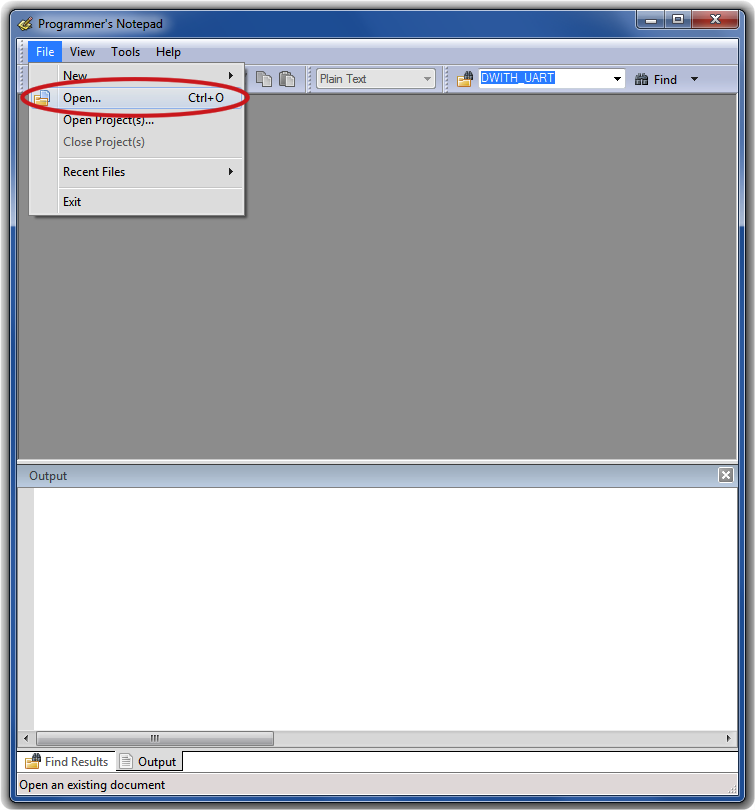
\includegraphics[width=.85\textwidth]{../PNG/Notepad_open.png}
    \caption{open Makefile}
  \end{subfigure}
  ~
  \begin{subfigure}[b]{.5\textwidth}
    \centering
    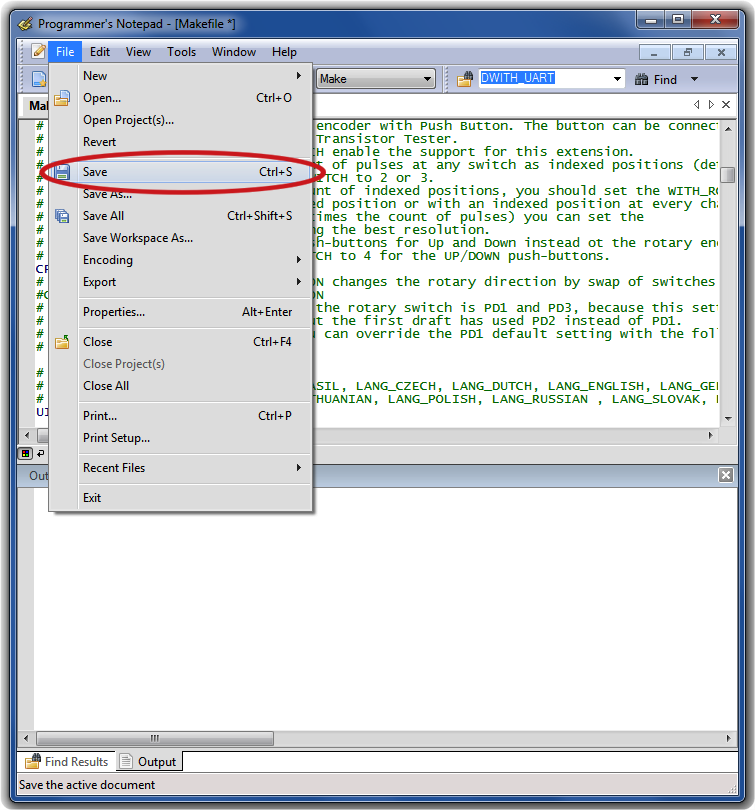
\includegraphics[width=.85\textwidth]{../PNG/Notepad_save.png}
    \caption{save Makefile}
  \end{subfigure}
  \caption{Bedienung der WinAVR-Oberfläche Programmer's Notepad}
  \label{fig:WinAVR1}
\end{figure}
Die Abbildungen \ref{fig:WinAVR1} zeigen das File-Menü der Bedienoberfläche von WinAVR zum
Öffnen der Datei \lname{Makefile} und zum Abspeichern der \lname{Makefile} nach den Änderungen (save).
\begin{figure}[H]
  \begin{subfigure}[b]{.5\textwidth}
    \centering
    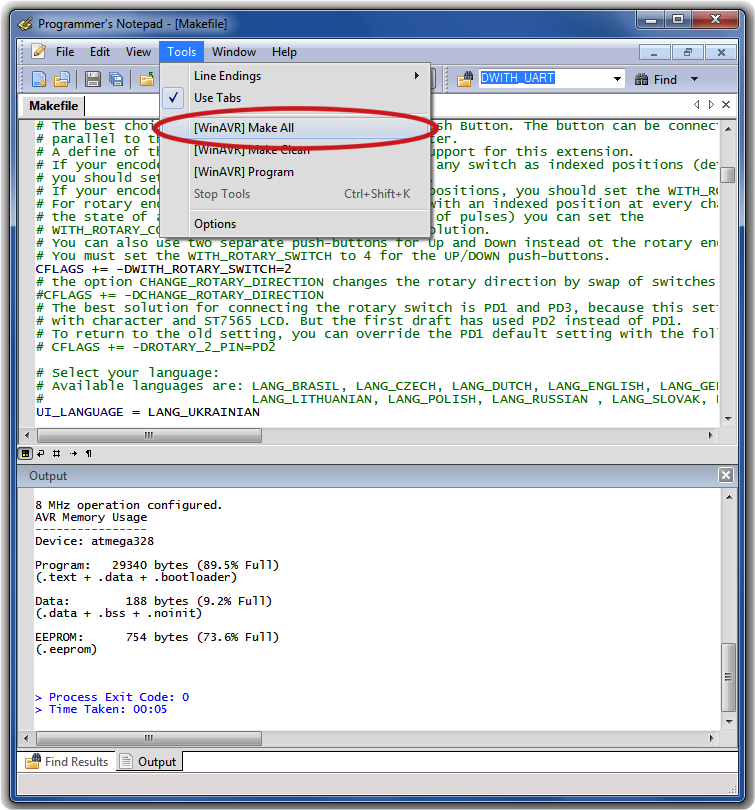
\includegraphics[width=.85\textwidth]{../PNG/Notepad_make.png}
    \caption{Erzeuge Programmdaten (.hex/.eep)}
  \end{subfigure}
  ~
  \begin{subfigure}[b]{.5\textwidth}
    \centering
    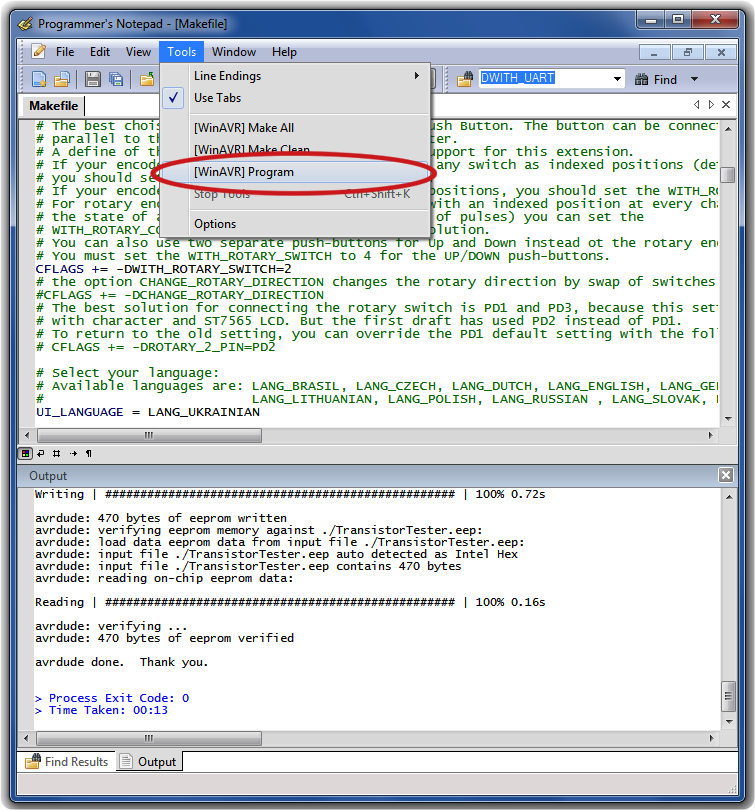
\includegraphics[width=.85\textwidth]{../PNG/Notepad_program.png}
    \caption{Programmiere ATmega}
  \end{subfigure}
  \caption{Bedienung der WinAVR-Oberfläche Programmer's Notepad}
  \label{fig:WinAVR2}
\end{figure}
Die nächsten Abbildungen \ref{fig:WinAVR2} zeigen das Tools-Menü von Programmer's Notepad
zum Übersetzen des Programms (Make All) und zum Programmieren des ATmega (Program) mit \lcmd{avrdude}.
